\documentclass[11pt,a4paper]{article}

\usepackage[T1]{fontenc}
\usepackage[utf8]{inputenc}
\usepackage[polish]{babel}
\usepackage{lmodern}
\usepackage[margin=2.5cm]{geometry}
\usepackage{microtype}
\usepackage{amsmath}
\usepackage{graphicx}
\usepackage{booktabs}
\usepackage{longtable}
\usepackage{array}
\usepackage{pdflscape}
\usepackage{caption}
\usepackage[hidelinks]{hyperref}

\graphicspath{{figures/}{../figures/}}
\captionsetup{font=small,labelfont=bf}
\setlength{\parskip}{0.3em}
\setlength{\parindent}{1.2em}

\newcommand{\pimin}{\ensuremath{\pi_{\mathrm{min}}}}
\newcommand{\pigold}{\ensuremath{\pi_{\mathrm{gold}}}}
\newcommand{\dom}[1]{\texttt{#1}}

\title{Ile polskich serwisów newsowych publikuje masowo teksty generowane przez AI?\\
\large Pomiar bez etykiet na 35 tysiącach artykułów z lat 2020-2025}
\author{Mikołaj Machalski \and Mikołaj Czachorowski \and Wojciech Makowski \and Jan Szyndlarewicz}
\date{10 listopada 2026}

\begin{document}
\maketitle

\begin{abstract}
\noindent Sprawdzamy, czy polskie serwisy informacyjne publikują masowo, czyli w co najmniej 20\% artykułów, teksty generowane przez modele językowe. Mamy 35\,628 artykułów z 45 serwisów, pobranych z Common Crawl dla lat 2020--2025, ale żadnych etykiet autorstwa. Nie klasyfikujemy więc pojedynczych tekstów, tylko mierzymy nadwyżkę na poziomie serwisu. Przyjmujemy, że artykuły z lat 2020--2022 napisali ludzie, ustawiamy na nich próg detektora (5\% fałszywych alarmów), dla każdego serwisu mierzymy wzrost odsetka oznaczonych tekstów po 2022 r. i przeliczamy go na udział AI estymatorem Rogana--Gladena. Czułość detektora szacujemy na 100 polskich artykułach i ich przeróbkach wykonanych przez GPT-4.1-mini. Pangram EditLens odróżnia przeróbki od oryginałów (AUC 0,88), a detektory zero-shot oparte na polskim modelu Bielik prawie wcale (AUC 0,49--0,56), choć na polskim zbiorze PolEval Śmigiel radzą sobie równie dobrze jak Pangram. Wybór detektora wyłącznie na podstawie Śmigiela prowadziłby więc do wniosku, że wzrostu prawie nie ma. Z 37 serwisów, które da się porównać przed i po 2022 r., w jednym (\dom{zmianynaziemi.pl}) nadwyżka tekstów ocenianych przez detektor jako generowane przez AI odpowiada co najmniej 29,8\% jego artykułów z lat 2023--2025 przy dowolnej czułości detektora, o ile nie zmienił się poziom fałszywych alarmów. Drugi serwis (\dom{goniec.pl}) spełnia kryterium przy czułości zmierzonej na przeróbkach, a trzy kolejne traktujemy jako kandydatów, bo wypadają w części wariantów analizy. Żaden z największych serwisów nie spełnia kryterium w analizie głównej. W całej, celowo dobranej próbie dolna granica udziału AI w latach 2023--2025 wynosi 4,0\% [2,4; 6,1], a wśród największych serwisów 1,8\% [0,3; 3,4].
\end{abstract}

\medskip
\noindent\textbf{Słowa kluczowe:} wykrywanie tekstów generowanych maszynowo, media polskie, estymacja udziału bez etykiet, Pangram, Common Crawl

\section{Wprowadzenie}

Od premiery ChatGPT (30 listopada 2022 r.) napisanie artykułu po polsku kosztuje ułamek grosza. Serwisy, które żyją z ruchu z wyszukiwarek i mediów społecznościowych, mają powód, żeby z tego korzystać. Pytamy, w ilu polskich serwisach da się to zmierzyć.

Podobne pomiary robiono już dla innych korpusów (sekcja~\ref{sec:prace}), ale nie dla polskich mediów i nie z wynikiem osobno dla każdego serwisu. Naszym celem jest właśnie taki pomiar: po polsku, bez etykiet i na poziomie pojedynczego serwisu.

Za treść generowaną przez AI uznajemy tekst, który w całości lub w przeważającej części napisał model, także jako przeróbkę cudzego materiału. Serwis jest masowy, jeśli co najmniej 20\% jego artykułów z lat 2023--2025 wygenerowała AI. Wrażliwość na tę definicję pokazujemy w sekcji~\ref{sec:odpornosc}. Nasz instrument mierzy jednak coś szerszego. Pangram EditLens uczono szacować \emph{stopień} udziału AI w tekście, łącznie z redakcją tekstu ludzkiego~\cite{editlens}, a tego, jak często przekracza próg na tekstach tylko poprawionych przez model, nie sprawdzaliśmy. Nadwyżka, którą mierzymy, może więc obejmować również teksty ludzkie mocno zredagowane przez AI. Dlatego wyniki opisujemy jako udział tekstów, które detektor ocenia jako generowane przez AI.

Stawiamy dwie hipotezy. Według pierwszej (H1) odsetek tekstów oznaczanych przez detektor jest po 2022 r. wyższy niż przed nim, i to ponad to, co tłumaczą losowość i dryf detektora. Druga (H2, główna) mówi, że co najmniej jeden serwis z próby spełnia definicję „masowo”. Ponieważ część próby dobraliśmy celowo spośród serwisów podejrzewanych o takie praktyki, H2 nie mówi nic o polskich mediach w ogóle. Odpowiada tylko na pytanie, czy zjawisko w tej skali da się w ogóle wykryć naszym instrumentem. Wynik negatywny byłby pełnoprawną odpowiedzią.

Wkład pracy jest trojaki.
\begin{enumerate}
\item Procedura szacowania udziału tekstów AI w pojedynczym serwisie bez etykiet: próg kalibrowany na tekstach sprzed ChatGPT, poziom bazowy każdego serwisu, estymator Rogana--Gladena z dwoma założeniami o czułości i reguła klasyfikacji ustalona przed obejrzeniem wyników.
\item Pokazanie, że wybór detektora decyduje o odpowiedzi. Detektory zero-shot na polskim modelu, równie dobre jak Pangram na zbiorze PolEval Śmigiel, nie odróżniają przeróbek GPT od oryginalnych polskich newsów, a w danych nie widzą prawie żadnego wzrostu.
\item Wyniki dla 37 polskich serwisów z lat 2020--2025 wraz z analizą ich odporności na dziewięć wariantów metody.
\end{enumerate}

\section{Prace pokrewne}\label{sec:prace}

\paragraph{Pomiar udziału AI w korpusach.} Hanley i Durumeric~\cite{hanley2024} zastosowali klasyfikator syntetycznych newsów do ponad 15 mln artykułów z 3074 anglojęzycznych serwisów. Między styczniem 2022 a majem 2023 udział tekstów syntetycznych rósł szybciej w serwisach dezinformacyjnych niż w głównym nurcie, i to głównie w małych serwisach. Russell i in.~\cite{russell2025} użyli Pangrama na amerykańskich gazetach i ocenili, że około 9\% nowo publikowanych artykułów powstało w części lub w całości z udziałem AI, częściej w małych tytułach lokalnych. Liang i in.~\cite{liang2024icml, liang2025} szacują udział tekstów zmodyfikowanych przez LLM w recenzjach konferencyjnych i pracach naukowych metodą rozkładową, bez klasyfikowania pojedynczych tekstów, i sprawdzają ją na tekstach sprzed premiery ChatGPT. Od tych prac różnimy się językiem, wynikiem osobno dla każdego serwisu i jawnie modelowaną czułością detektora.

\paragraph{Estymacja udziału przy niedoskonałym klasyfikatorze.} Nasz estymator to w epidemiologii poprawka Rogana--Gladena~\cite{rogan}, a w uczeniu maszynowym metoda \emph{adjusted classify and count} z literatury o kwantyfikacji~\cite{forman2008, gonzalez2017}. W obu tradycjach odsetek pozytywnych wyników testu koryguje się znanymi odsetkami fałszywych alarmów i trafień. Problemy, z którymi się mierzymy, też są tam znane. Gdy czułość zmierzona na danych walidacyjnych nie przenosi się na dane docelowe, estymator jest obciążony, a gdy mianownik $\mathrm{TPR}-b$ jest mały, staje się bardzo niestabilny.

\paragraph{Detektory i ich przenośność.} Metody zero-shot oceniają, jak przewidywalny jest tekst dla modelu językowego: DetectGPT~\cite{detectgpt} przez krzywiznę log-prawdopodobieństwa, Fast-DetectGPT~\cite{fastdetectgpt} przez jej szybkie przybliżenie, Binoculars~\cite{binoculars} przez stosunek perplexity dwóch modeli. Detektory uczone, jak Pangram EditLens~\cite{editlens}, przewidują stopień udziału AI w tekście. Benchmark RAID~\cite{raid} pokazał, że skuteczność detektorów silnie zależy od dziedziny i że domyślne progi dają wysokie odsetki fałszywych alarmów. Dla polskiego najbliższym punktem odniesienia jest zadanie Śmigiel z PolEval 2025~\cite{smigiel} i modele Bielik~\cite{bielik}. Według naszej wiedzy nikt dotąd nie porównał tych detektorów na polskich newsach przerobionych przez model komercyjny.

\section{Dane}

\subsection{Rama próby i pobieranie}

Rama ma 50 domen w trzech warstwach. S1 to 12 największych polskich serwisów informacyjnych według rankingu Tranco~\cite{tranco}, S2 to 24 dalsze serwisy z rankingu, w tym regionalne, a S3 to 14 serwisów spoza rankingu, dodanych ręcznie. Są wśród nich serwisy regionalne oraz „alternatywne” i konspiracyjne, które wybraliśmy celowo, bo podejrzewaliśmy je o interesujące nas praktyki. Próba nie jest więc losowa i wnioski dotyczą tylko tych serwisów. Wyniki podajemy także osobno dla warstw.

Artykuły pobraliśmy z Common Crawl~\cite{cc}, z jednego crawla na rok publikacji (od CC-MAIN-2021-04 dla 2020 r. do CC-MAIN-2026-04 dla 2025 r.), z kwotą 200 artykułów na serwis i rok. Tekst i datę publikacji wyciągnęła biblioteka trafilatura~\cite{trafilatura}. Zostawiliśmy artykuły z co najmniej 150 słowami, znacznikami artykułu w HTML i datą z danego roku. Po usunięciu 195 powtórzonych tekstów zostało 35\,628 artykułów z 45 serwisów (pięć domen z ramy nie dało nic), rozłożonych na lata tak, jak pokazuje tabela~\ref{tab:pokrycie} i rysunek~\ref{fig:pokrycie}.

\begin{table}[t]
\centering\small
\caption{Liczba artykułów i serwisów z danymi w kolejnych latach.}\label{tab:pokrycie}
\begin{tabular}{@{}lrrrrrrr@{}}
\toprule
 & 2020 & 2021 & 2022 & 2023 & 2024 & 2025 & razem \\
\midrule
artykuły & 7\,178 & 7\,127 & 6\,509 & 6\,178 & 4\,855 & 3\,781 & 35\,628 \\
serwisy z danymi & 41 & 43 & 41 & 42 & 35 & 30 & 45 \\
\bottomrule
\end{tabular}
\end{table}

\begin{figure}[t]
\centering
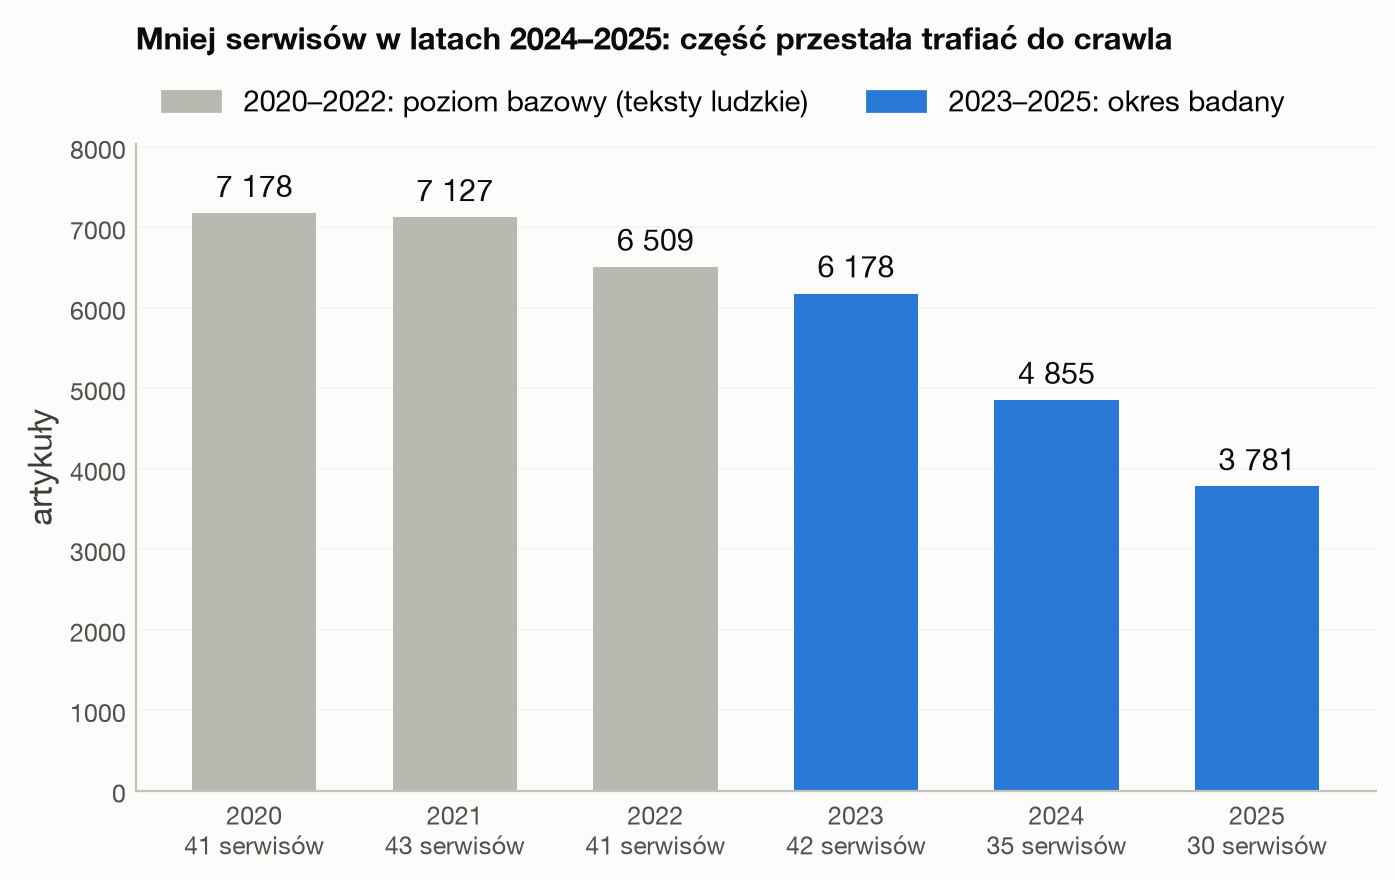
\includegraphics[width=0.85\linewidth]{fig01_coverage.png}
\caption{Liczba artykułów i serwisów z danymi w kolejnych latach. Pełna tabela serwis $\times$ rok jest w repozytorium (\texttt{figures/fig01b\_coverage\_heatmap}).}\label{fig:pokrycie}
\end{figure}

\subsection{Nierówne pokrycie i wyłączenia}

Pokrycie jest nierówne. Grupa regionalnych serwisów jednego wydawcy (np. \dom{dzienniklodzki.pl}, \dom{gs24.pl}, \dom{pomorska.pl}) i \dom{radiozet.pl} mają po 200 tekstów do 2023 r., a w latach 2024--2025 nie ma ich w crawlu. Porównanie „wszystkie teksty przed i wszystkie po” mieszałoby więc zmianę w czasie ze zmianą składu serwisów. Każdy serwis porównujemy dlatego z nim samym, a wynik zbiorczy liczymy z poprawką na skład (sekcja~\ref{sec:niepewnosc}).

Do porównania wchodzi serwis, który ma co najmniej 50 tekstów w każdym okresie. Spełnia to 37 serwisów. Osiem pozostałych (tab.~\ref{tab:wylaczone}) opisujemy osobno, bez wniosków o udziale AI, bo bez poziomu bazowego serwisu nie wiadomo, czy wysoki odsetek oznaczonych to AI, czy cecha jego tekstów. Sześć z nich należy do S3, więc porównywalnych serwisów S3 jest tylko siedem.

\begin{table}[t]
\centering\small
\caption{Serwisy wyłączone z porównania przed/po.}\label{tab:wylaczone}
\begin{tabular}{@{}llrrl@{}}
\toprule
serwis & warstwa & $n$ 2020--22 & $n$ 2023--25 & powód \\
\midrule
\dom{gazeta.pl} & S1 & 583 & 24 & za mało po 2022 r. \\
\dom{wyborcza.pl} & S2 & 4 & 24 & za mało w obu okresach \\
\dom{neon24.pl} & S3 & 7 & 215 & brak poziomu bazowego \\
\dom{wpolsce24.tv} & S3 & 0 & 358 & brak poziomu bazowego \\
\dom{odkrywamyzakryte.com} & S3 & 400 & 0 & brak danych po 2022 r. \\
\dom{tvp.info} & S3 & 600 & 0 & brak danych po 2022 r. \\
\dom{parezja.pl} & S3 & 167 & 10 & za mało po 2022 r. \\
\dom{pikio.pl} & S3 & 270 & 16 & za mało po 2022 r. \\
\bottomrule
\end{tabular}
\end{table}

\section{Pomiar}

\subsection{Detektory i dane odniesienia}

Głównym kandydatem był Pangram EditLens~\cite{editlens}, klasyfikator zbudowany na modelu Llama-3.2-3B z adapterem LoRA, który zwraca wynik od 0 do 1 (1024 tokeny). Uczono go głównie na tekstach angielskich. Drugą grupą są metody zero-shot na polskim modelu Bielik~\cite{bielik} (wersje 1,5B i 4,5B v3, 512 tokenów): Binoculars~\cite{binoculars} i Fast-DetectGPT~\cite{fastdetectgpt}, a dla porównania zwykła perplexity. Zero-shot były naszym pierwszym wyborem, bo nie wymagają danych uczących i działają w języku badanych serwisów.

Detektory sprawdzamy na dwóch zbiorach. Pierwszy to Śmigiel z PolEval 2025~\cite{smigiel}: 1000 polskich tekstów, w tym 500 z modeli open-source. Są bardzo krótkie (mediana 49 słów) i nie są newsami. Drugi, własny zbiór gold, ma przypominać badane dane. Jego część G1 to 100 ludzkich artykułów z 2020 r. z 24 naszych serwisów, o długości 200--1500 słów, losowanych kolejno z każdego serwisu. Automatycznie odrzuciliśmy reklamy, artykuły sponsorowane, komunikaty prawne, listy i tabele, a po przeczytaniu jeszcze 14 tekstów ręcznie. Część G2 to te same 100 artykułów napisane od nowa przez \texttt{gpt-4.1-mini} (temperatura 0,7). Polecenie brzmiało: napisać artykuł własnymi słowami, „jak dla redakcji, która przerabia cudzy materiał na własny”, z zachowaniem faktów, nazwisk, liczb i cytatów, w długości 80--120\% oryginału. Odpowiedzi kopiujące więcej niż 25\% 5-gramów oryginału oznaczaliśmy. Pary mają ten sam temat i podobną długość, więc różnica w wyniku detektora nie wynika z tych cech. Przeróbki zachowują cytaty oryginału, są więc częściowo tekstem ludzkim. Czułość na G2 to czułość na mocno przerobione teksty ludzkie, a nie na teksty pisane przez model od zera. Wyniki Pangrama dla G1 w zbiorze gold i w naszych danych są prawie identyczne (mediana różnicy 0,002, korelacja rang 0,87), więc progi z naszych danych można stosować do gold.

\subsection{Wybór detektora}

Tabela~\ref{tab:auc} i rysunek~\ref{fig:auc} pokazują rozdźwięk. Detektory Bielika radzą sobie na Śmigielu równie dobrze jak Pangram (AUC 0,79--0,84 wobec 0,80), ale na przeróbkach GPT w polskich newsach nie odróżniają przeróbki od oryginału (AUC 0,49--0,56). Skoro na Śmigielu nie są gorsze, to ich ślepota na zbiorze gold nie wygląda na błąd implementacji. Najprawdopodobniej mierzą, jak przewidywalny jest tekst dla Bielika, a przeróbka GPT, która zachowuje fakty, nazwiska i cytaty oryginału, jest dla Bielika tak samo przewidywalna jak on sam. Zwykła perplexity ma przyzwoite AUC (0,77), ale przy naszym progu nie oznacza prawie niczego (TPR 1\%).

Główną analizę prowadzimy więc na Pangramie. Zdecydowała walidacja. To, jaki wynik detektor daje na badanych danych, nie miało wpływu na wybór. Zbiór gold policzyliśmy tylko dla Bielika 1,5B, a w danych używamy wersji 4,5B z oknem 512 tokenów. Na Śmigielu wersja 4,5B daje prawie te same krzywe, więc zakładamy, bez bezpośredniego sprawdzenia, że ślepota dotyczy też jej.

\begin{table}[t]
\centering\small
\caption{Walidacja detektorów. AUC na Śmigielu i na zbiorze gold (z 95\% przedziałem), odsetek par, w których przeróbka ma wyższy wynik niż oryginał, oraz czułość na G2 przy progu z FPR 5\%.}\label{tab:auc}
\begin{tabular}{@{}p{5.6cm}cccc@{}}
\toprule
detektor & AUC Śmigiel & AUC gold & przeróbka wyżej & TPR (G2) \\
\midrule
Pangram EditLens & 0,80 & \textbf{0,88} [0,83; 0,92] & 89\% & \textbf{26\%} \\
Binoculars (Bielik 1,5B) & 0,84 & 0,56 [0,50; 0,62] & 56\% & 2\% \\
Fast-DetectGPT, bazowy (1,5B) & 0,79 & 0,49 [0,43; 0,56] & 43\% & 4\% \\
Fast-DetectGPT, instrukcyjny (1,5B) & 0,80 & 0,56 [0,50; 0,63] & 54\% & 11\% \\
zwykła perplexity (1,5B) & 0,71 & 0,77 [0,72; 0,81] & 92\% & 1\% \\
\bottomrule
\end{tabular}
\end{table}

\begin{figure}[t]
\centering
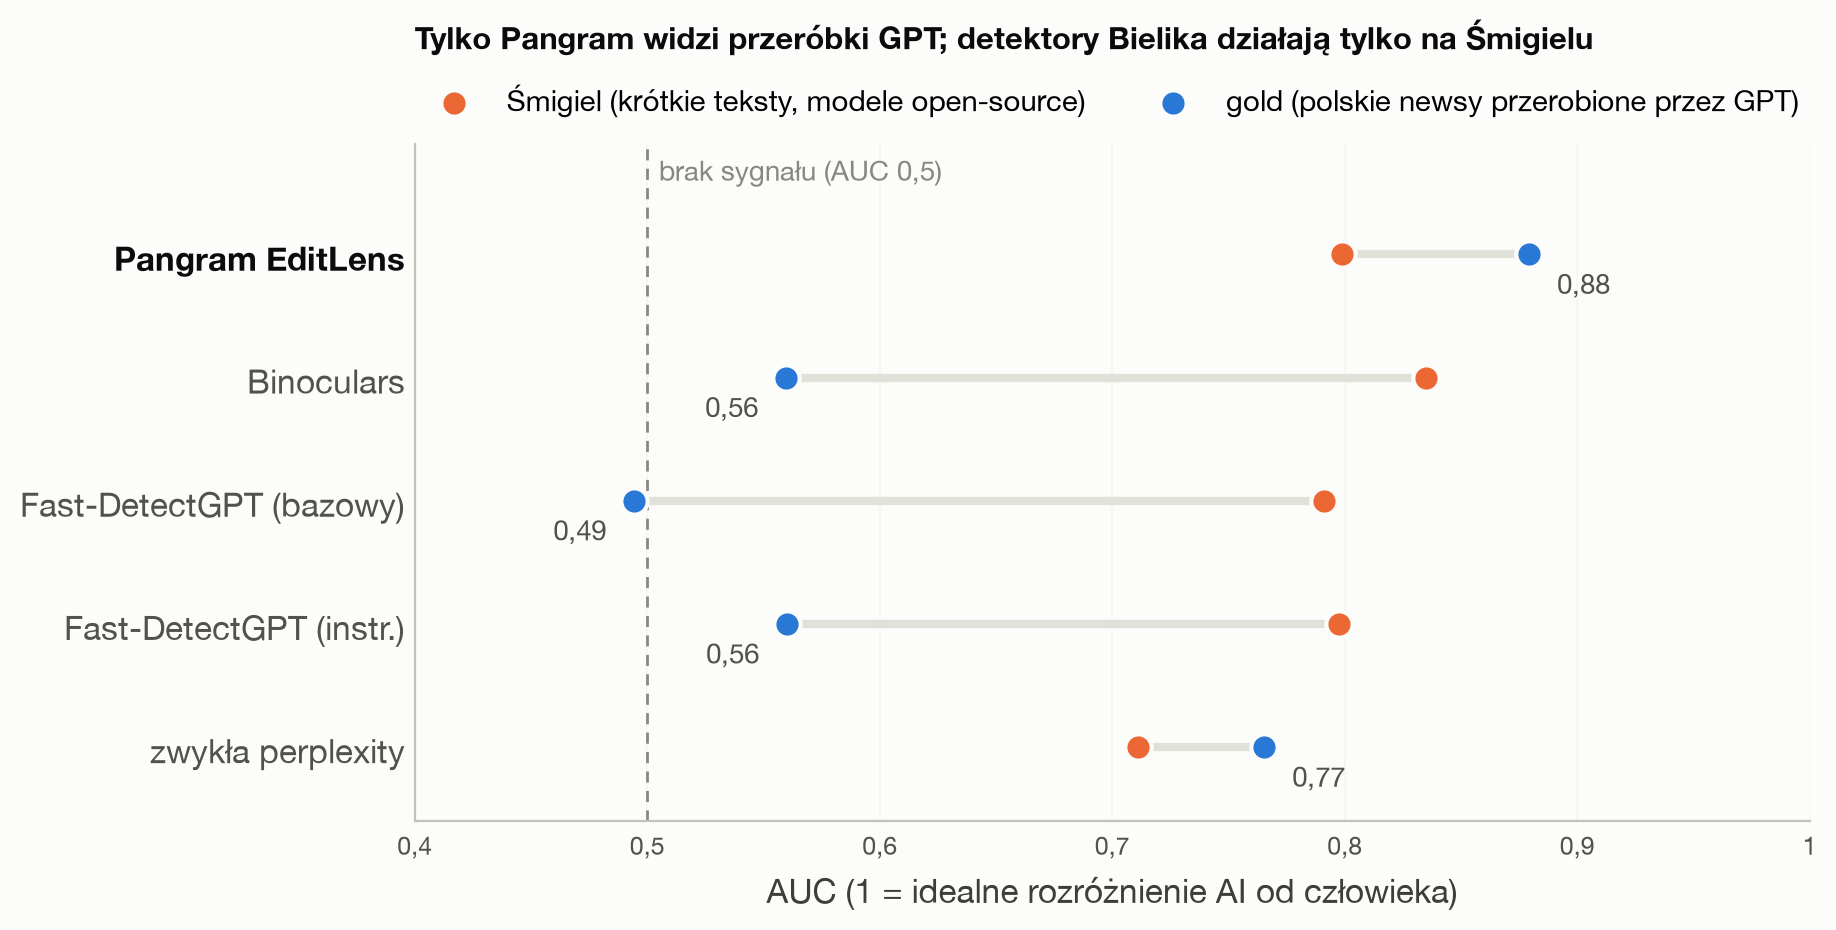
\includegraphics[width=\linewidth]{fig02_instrument_auc.png}
\caption{AUC na dwóch zbiorach odniesienia. Detektory Bielika działają na tekstach z modeli open-source (Śmigiel), ale nie widzą przeróbek GPT w polskich newsach (gold). Krzywe ROC są w repozytorium (\texttt{figures/fig02b\_roc}).}\label{fig:auc}
\end{figure}

\subsection{Próg, czułość i wybór FPR 5\%}\label{sec:prog}

Próg ustawiamy na tekstach z lat 2020--2022 ze zbiorów \texttt{train} i \texttt{dev} (18\,732 teksty), tak by 5\% z nich leżało powyżej (0,472 w skali Pangrama). Na odłożonym zbiorze \texttt{test} (2\,082 teksty), którego nie użyliśmy do ustawienia progu, oznaczonych jest 4,4\% [3,6; 5,3]. Wśród 100 ludzkich tekstów G1 oznaczonych jest 6\%, ale G1 pochodzi z naszych danych z 2020 r., więc w większości należy do zbioru kalibracyjnego i nie jest sprawdzeniem poza próbą. Ten sam próg daje na przeróbkach G2 TPR = 26\% [18,4; 35,4], czyli 26 ze 100. AUC jest wysokie, bo przeróbki mają zwykle wyższy wynik niż oryginały, ale rzadko przekraczają próg ustawiony na najbardziej „AI-podobnych” 5\% tekstów ludzkich (rys.~\ref{fig:prog}).

\begin{figure}[t]
\centering
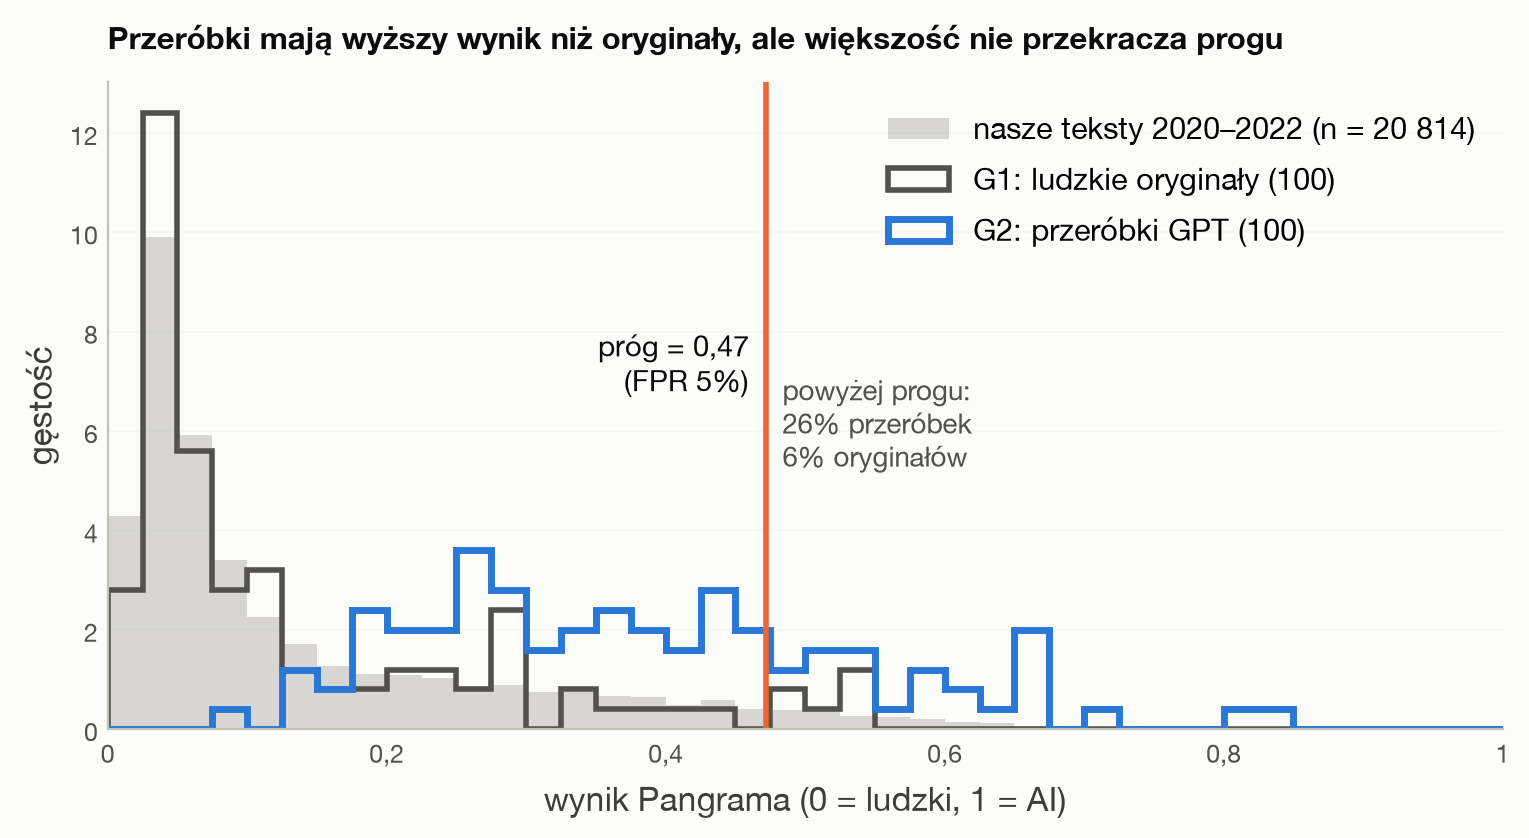
\includegraphics[width=0.9\linewidth]{fig03_threshold_hist.png}
\caption{Rozkład wyniku Pangrama dla naszych tekstów z lat 2020-2022, ludzkich oryginałów G1 i przeróbek G2.}\label{fig:prog}
\end{figure}

Stały FPR i kalibracja na tekstach ludzkich z tej samej dziedziny to praktyka znana z benchmarku RAID~\cite{raid}. Każdemu detektorowi ustawiano tam próg tak, by 5\% tekstów ludzkich było błędnie oznaczonych. Autorzy pokazali, że domyślne progi dają w otwartych detektorach bardzo wysoki odsetek fałszywych alarmów, a jeden próg globalny daje w poszczególnych dziedzinach wyraźnie różny FPR. Z tego drugiego wniosku wynika nasz układ: próg jest jeden, ale poziom bazowy $b$ mierzymy osobno dla każdego serwisu.

Wartość 5\% jest konwencją i nie twierdzimy, że jest optymalna. Przy 1\% Pangram wykrywa tylko 10\% przeróbek, więc nadwyżka w serwisie byłaby ułamkiem punktu procentowego, a każdy błąd mnożyłby się przez $1/(\mathrm{TPR}-b)\approx 11$. Przy 10-20\% czułość rośnie, ale próg schodzi w środek rozkładu tekstów ludzkich, gdzie wynik silniej zależy od gatunku i długości tekstu, i rośnie dryf (margines dryfu z 2,9 pp przy 5\% do 9,6 pp przy 20\%). Poziom 5\% przyjęliśmy przed obejrzeniem wyników dla serwisów, a wyniki dla 1, 10 i 20\% pokazujemy w sekcji~\ref{sec:fpr}.

\subsection{Estymator}\label{sec:estymator}

Dla serwisu znamy trzy wielkości: $b$, czyli odsetek oznaczonych tekstów w latach 2020-2022 (fałszywe alarmy na tekstach ludzkich tego serwisu), $r$, czyli ten sam odsetek w latach 2023-2025, oraz TPR. Jeśli udział AI wynosi $\pi$, to $r=\pi\cdot\mathrm{TPR}+(1-\pi)\,b$, skąd
\begin{equation}
\pi=\frac{r-b}{\mathrm{TPR}-b},
\end{equation}
obcięte do przedziału $[0,1]$. To estymator Rogana-Gladena~\cite{rogan}, którego epidemiolodzy używają do szacowania częstości choroby testem o znanej czułości i swoistości. Pojedynczy oznaczony artykuł niczego nie dowodzi, bo przy FPR 5\% co dwudziesty tekst ludzki też jest oznaczony. Wnioskujemy wyłącznie o nadwyżce na poziomie serwisu.

Czułość znamy tylko dla przeróbek GPT-4.1-mini. Dla tekstów, które serwisy faktycznie publikują (inny model, pisanie od zera, tłumaczenie, poprawki człowieka), może być inna. Podajemy więc dwa szacunki. \pimin{} przyjmuje TPR = 100\%. Detektor nie wykryje więcej niż wszystkich tekstów AI, więc \pimin{} jest dolną granicą prawdziwego udziału, ale tylko warunkowo: przy założeniu, że bez AI poziom bazowy serwisu by się nie zmienił, a artykuły są od siebie niezależne. \pigold{} przyjmuje TPR = 26\% z przeróbek G2. Jest realistyczny, jeśli teksty AI w serwisie są równie trudne do wykrycia jak przeróbki, a dla tekstów łatwiejszych do wykrycia, np. generowanych od zera, udział przeszacowuje. \pigold{} traktujemy więc jako szacunek warunkowy, a nie górną granicę, bo górnej granicy udziału nie identyfikujemy. Gdy odsetek oznaczonych w serwisie przekracza TPR, model z TPR z G2 nie może opisywać danych i \pigold{} wychodzi powyżej 100\%. Obcinamy go wtedy do 100\% i oznaczamy w tabelach jako „$>$100”. Oznacza to, że teksty AI w tym serwisie są łatwiejsze do wykrycia niż nasze przeróbki.

\subsection{Margines dryfu}\label{sec:dryf}

Estymator zakłada, że bez AI odsetek oznaczonych by się nie zmienił. Detektor może jednak reagować na zmianę tematów, stylu albo szablonu strony. W serwisach, które mają co najmniej 50 tekstów w danym roku, porównujemy więc jeden rok z lat 2020--2022 z dwoma pozostałymi (razem 110 porównań). AI nie było w żadnym z nich, więc każda różnica to losowość albo dryf. Za margines $\delta$ przyjmujemy 95.\ percentyl tych różnic, czyli 2,9 punktu procentowego (pp). Nadwyżkę serwisu uznajemy za coś więcej niż szum dopiero wtedy, gdy przekracza $\delta$.

Margines ma trzy ograniczenia, które trzeba nazwać wprost. Po pierwsze, łączy dryf i zwykły szum losowania i ich nie rozdziela. Placebo pokazuje tylko, że w latach 2020--2022 zmiany są małe, a nie, ile z nich to dryf. Po drugie, $\delta$ jest jedną liczbą dla wszystkich serwisów, choć szum zależy od ich liczby tekstów, więc dla małych serwisów kryterium jest łagodniejsze. Po trzecie, dla grup „masowych” warunek nadwyżka $>\delta$ nie jest wiążący, bo dolna granica udziału $\geq 20\%$ i tak wymusza nadwyżkę znacznie większą od $\delta$. O tym, czy serwis jest masowy, decyduje więc dolna granica przedziału, a $\delta$ oddziela tylko serwisy bez żadnego sygnału. Placebo nie wykryje też zmiany, która zaczęła się dopiero po 2022 r. (sekcja~\ref{sec:ograniczenia}).

\subsection{Niepewność i reguła klasyfikacji}\label{sec:niepewnosc}

Przedziały dla serwisów liczymy symulacją, która w 5000 powtórzeń losuje jednocześnie $r$, $b$ i TPR. Każdy z tych odsetków $k/n$ losujemy z rozkładu Beta$(k+\tfrac12,\,n-k+\tfrac12)$, czyli rozkładu a posteriori przy priorze Jeffreysa~\cite{brown2001}. Dla TPR jest to 26 trafień na 100 przeróbek G2. Przy 5000 powtórzeniach 5.\ percentyl ma błąd Monte Carlo rzędu kilku dziesiątych punktu procentowego, więc serwisy z dolną granicą w odległości mniejszej niż ok. 1 pp od progu traktujemy jako graniczne. Wynik zbiorczy liczymy z poprawką na skład: poziom bazowy dopasowujemy do serwisów po 2022 r., z wagą równą liczbie ich tekstów z lat 2023--2025. Niepewność wynika z losowania serwisów ze zwracaniem i losowania TPR.

Poziom przedziałów jest w różnych miejscach różny i ma to uzasadnienie. Dla wyniku zbiorczego i liczb opisowych (TPR, FPR, odsetki rok po roku, AUC) podajemy zwykły przedział dwustronny 95\%. Dla serwisu reguła zadaje pytanie jednostronne, czy udział AI wynosi \emph{co najmniej} 20\%, więc liczy się tylko dolna granica. Dolny koniec przedziału 5.--95.\ percentyl jest jednostronną granicą ufności 95\%, spójną z $\delta$, które też jest 95.\ percentylem. Górny koniec służy do rysowania. Przedział 95\% dwustronny dawałby dla serwisu test na poziomie 2,5\%, ostrzejszy, niż wynika z pytania. Pokrycie dolnej granicy sprawdzamy symulacją w sekcji~\ref{sec:pokrycie}. Przedziały dla serwisów podpisujemy „90\% CI”.

Serwis trafia do jednej z czterech grup (tab.~\ref{tab:regula}). Regułę ustaliliśmy przed obejrzeniem wyników dla poszczególnych serwisów. Za odpowiedź na pytanie badawcze uznajemy tylko te, które są „masowe” we wszystkich wariantach analizy odporności.

\begin{table}[t]
\centering\small
\caption{Reguła klasyfikacji serwisu.}\label{tab:regula}
\begin{tabular}{@{}p{3.6cm}p{11cm}@{}}
\toprule
grupa & warunek \\
\midrule
masowo: mocne dowody & nadwyżka $>\delta$ i dolna granica 90\% CI dla \pimin{} $\geq 20\%$ \\
masowo: prawdopodobnie & nadwyżka $>\delta$ i dolna granica 90\% CI dla \pigold{} $\geq 20\%$ (ale nie powyższe) \\
nadwyżka poniżej progu & nadwyżka $>\delta$, ale żaden z powyższych warunków \\
brak nadwyżki ponad dryf & nadwyżka $\leq\delta$ \\
\bottomrule
\end{tabular}
\end{table}

\section{Wyniki}

\subsection{Stabilność detektora w latach bez AI}

W latach 2020--2022 odsetek oznaczonych jest płaski (4,8\%, 5,1\%, 4,9\%), także w panelu 16 serwisów, które mają dane w każdym roku (4,6\%, 4,4\%, 5,0\%). W tym stałym składzie wzrost zaczyna się dopiero w 2024 r. (4,0\% w 2023, 7,1\% w 2024, 8,5\% w 2025). Wzrost widoczny w 2023 r. we wszystkich serwisach razem (7,1\%) pochodzi więc z serwisów spoza stałego składu, między innymi \dom{zmianynaziemi.pl} i \dom{neon24.pl} (rys.~\ref{fig:lata}).

W teście placebo zmiany w serwisach bez AI są małe i symetryczne wokół zera (mediana +0,2 pp, 95.\ percentyl +2,9 pp). Po 2022 r. rozkład przesuwa się w prawo (mediana +2,5 pp), a 17 z 37 serwisów ma nadwyżkę większą niż $\delta$ (rys.~\ref{fig:placebo}). Ta kontrola wyklucza dryf detektora z roku na rok, ale nie wyklucza dryfu, który zaczął się dokładnie po 2022 r. z innego powodu (sekcja~\ref{sec:ograniczenia}).

\begin{figure}[t]
\centering
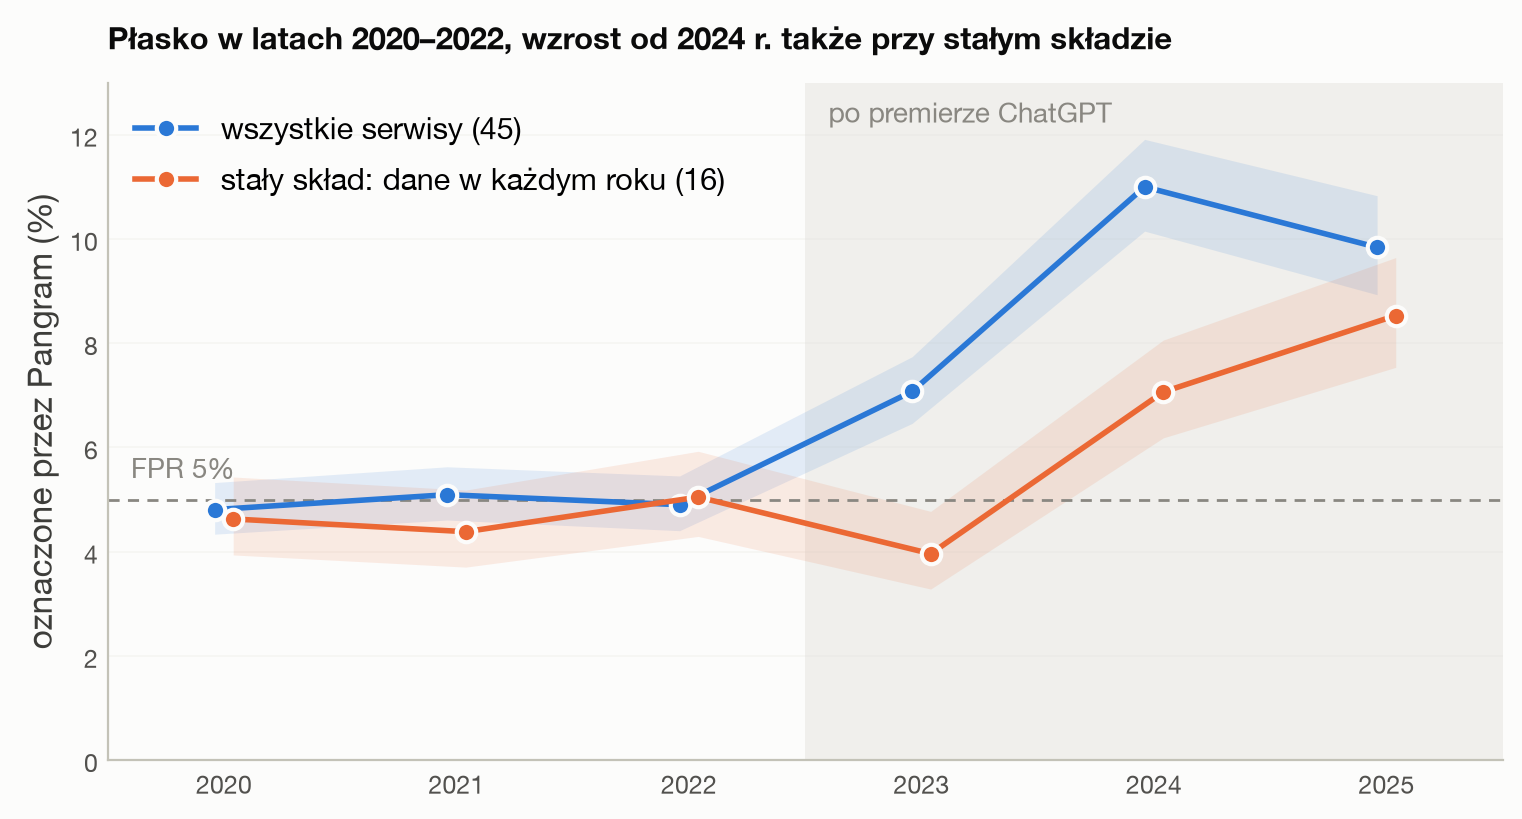
\includegraphics[width=0.9\linewidth]{fig04_yearly.png}
\caption{Odsetek tekstów oznaczonych przez Pangram (FPR 5\%) w kolejnych latach. Pasma: 95\% przedział Wilsona.}\label{fig:lata}
\end{figure}

\begin{figure}[t]
\centering
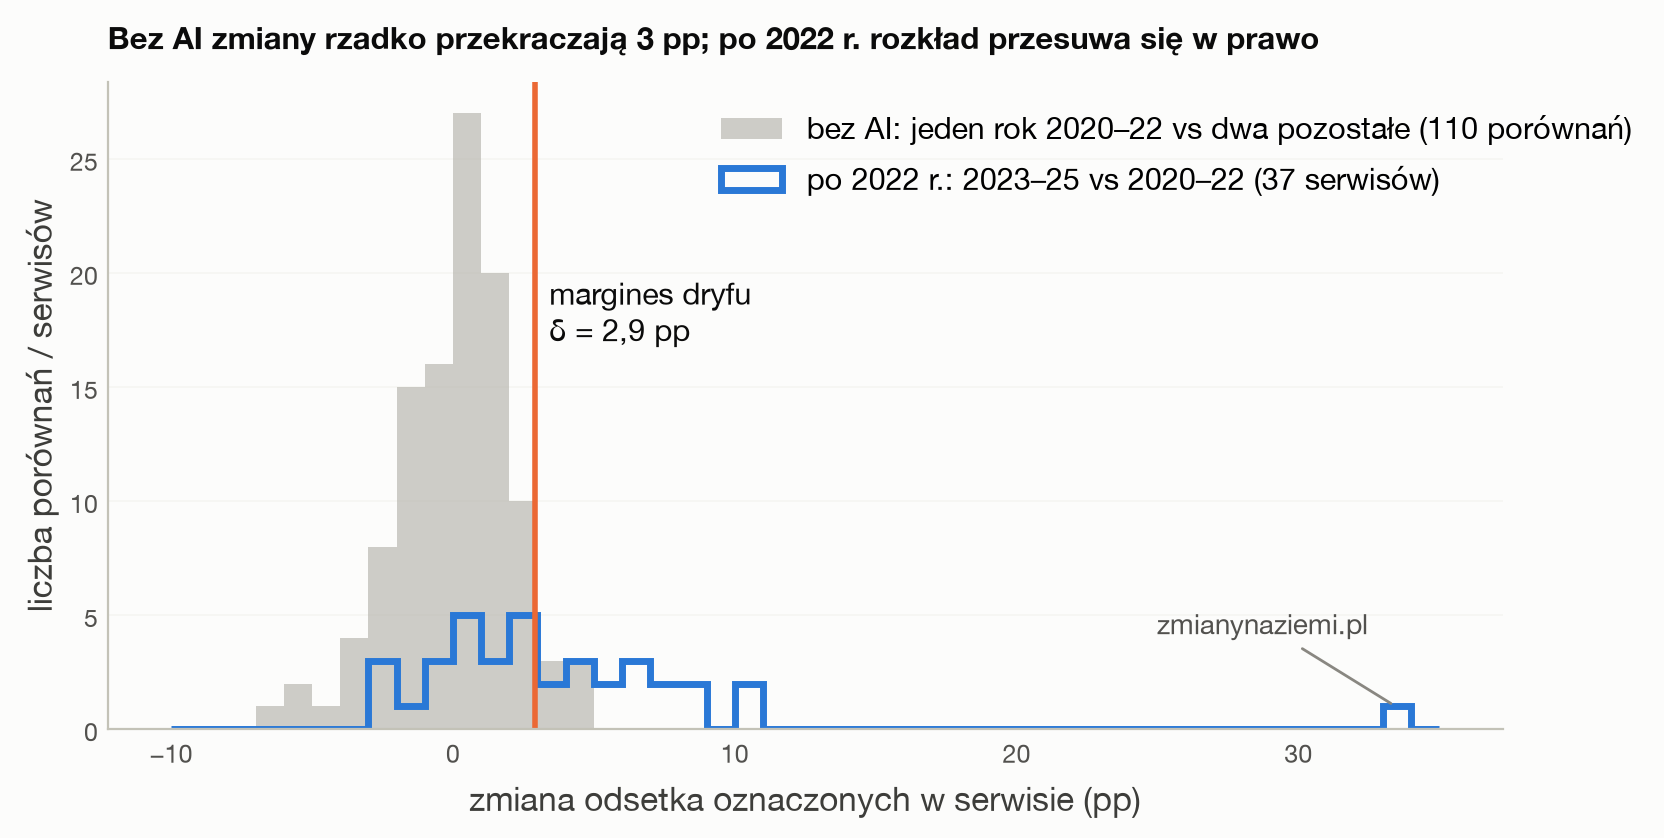
\includegraphics[width=0.9\linewidth]{fig05_placebo.png}
\caption{Zmiany odsetka oznaczonych w serwisach bez AI (placebo, 2020--2022) i po 2022 r.}\label{fig:placebo}
\end{figure}

\subsection{Wynik zbiorczy}

\begin{table}[t]
\centering\small
\caption{Wynik zbiorczy z poprawką na skład serwisów. Przedziały 95\%.}\label{tab:zbiorczy}
\begin{tabular}{@{}lrrrrll@{}}
\toprule
okres & teksty & poziom bazowy & oznaczone & nadwyżka & \pimin{} & \pigold{} \\
\midrule
2023 & 5\,948 & 4,7\% & 5,7\% & +0,9 pp & 1,0\% [0,0; 2,1] & 4,3\% [0,0; 10,7] \\
2024 & 4\,673 & 4,9\% & 11,0\% & +6,1 pp & 6,4\% [3,2; 11,6] & 29,0\% [13,1; 59,2] \\
2025 & 3\,546 & 4,5\% & 10,2\% & +5,8 pp & 6,1\% [3,0; 10,0] & 26,8\% [12,3; 51,9] \\
\textbf{2023--2025} & \textbf{14\,167} & \textbf{4,7\%} & \textbf{8,6\%} & \textbf{+3,8 pp} & \textbf{4,0\% [2,4; 6,1]} & \textbf{18,1\% [9,7; 32,2]} \\
\bottomrule
\end{tabular}
\end{table}

H1 się potwierdza (tab.~\ref{tab:zbiorczy}). Udział tekstów AI w latach 2023--2025 szacujemy na od co najmniej 4\% do około 18\%. W 2023 r. nadwyżka jest mała, a przedział \pigold{} obejmuje zero, w latach 2024--2025 jest wyraźna. Zjawisko narasta więc z opóźnieniem względem premiery ChatGPT. Przedziały są szerokie, bo czułość znamy ze 100 przeróbek, i to jest główne źródło niepewności w całym badaniu.

\subsection{Wyniki dla serwisów}\label{sec:serwisy}

\begin{table}[t]
\centering\small
\caption{Liczba serwisów w grupach, według warstw.}\label{tab:grupy}
\begin{tabular}{@{}lrrrr@{}}
\toprule
grupa & S1 & S2 & S3 & razem \\
\midrule
masowo: mocne dowody & 0 & 1 & 0 & \textbf{1} \\
masowo: prawdopodobnie & 0 & 2 & 2 & \textbf{4} \\
nadwyżka poniżej progu & 4 & 5 & 3 & 12 \\
brak nadwyżki ponad dryf & 7 & 11 & 2 & 20 \\
razem & 11 & 19 & 7 & 37 \\
\bottomrule
\end{tabular}
\end{table}

\begin{figure}[p]
\centering
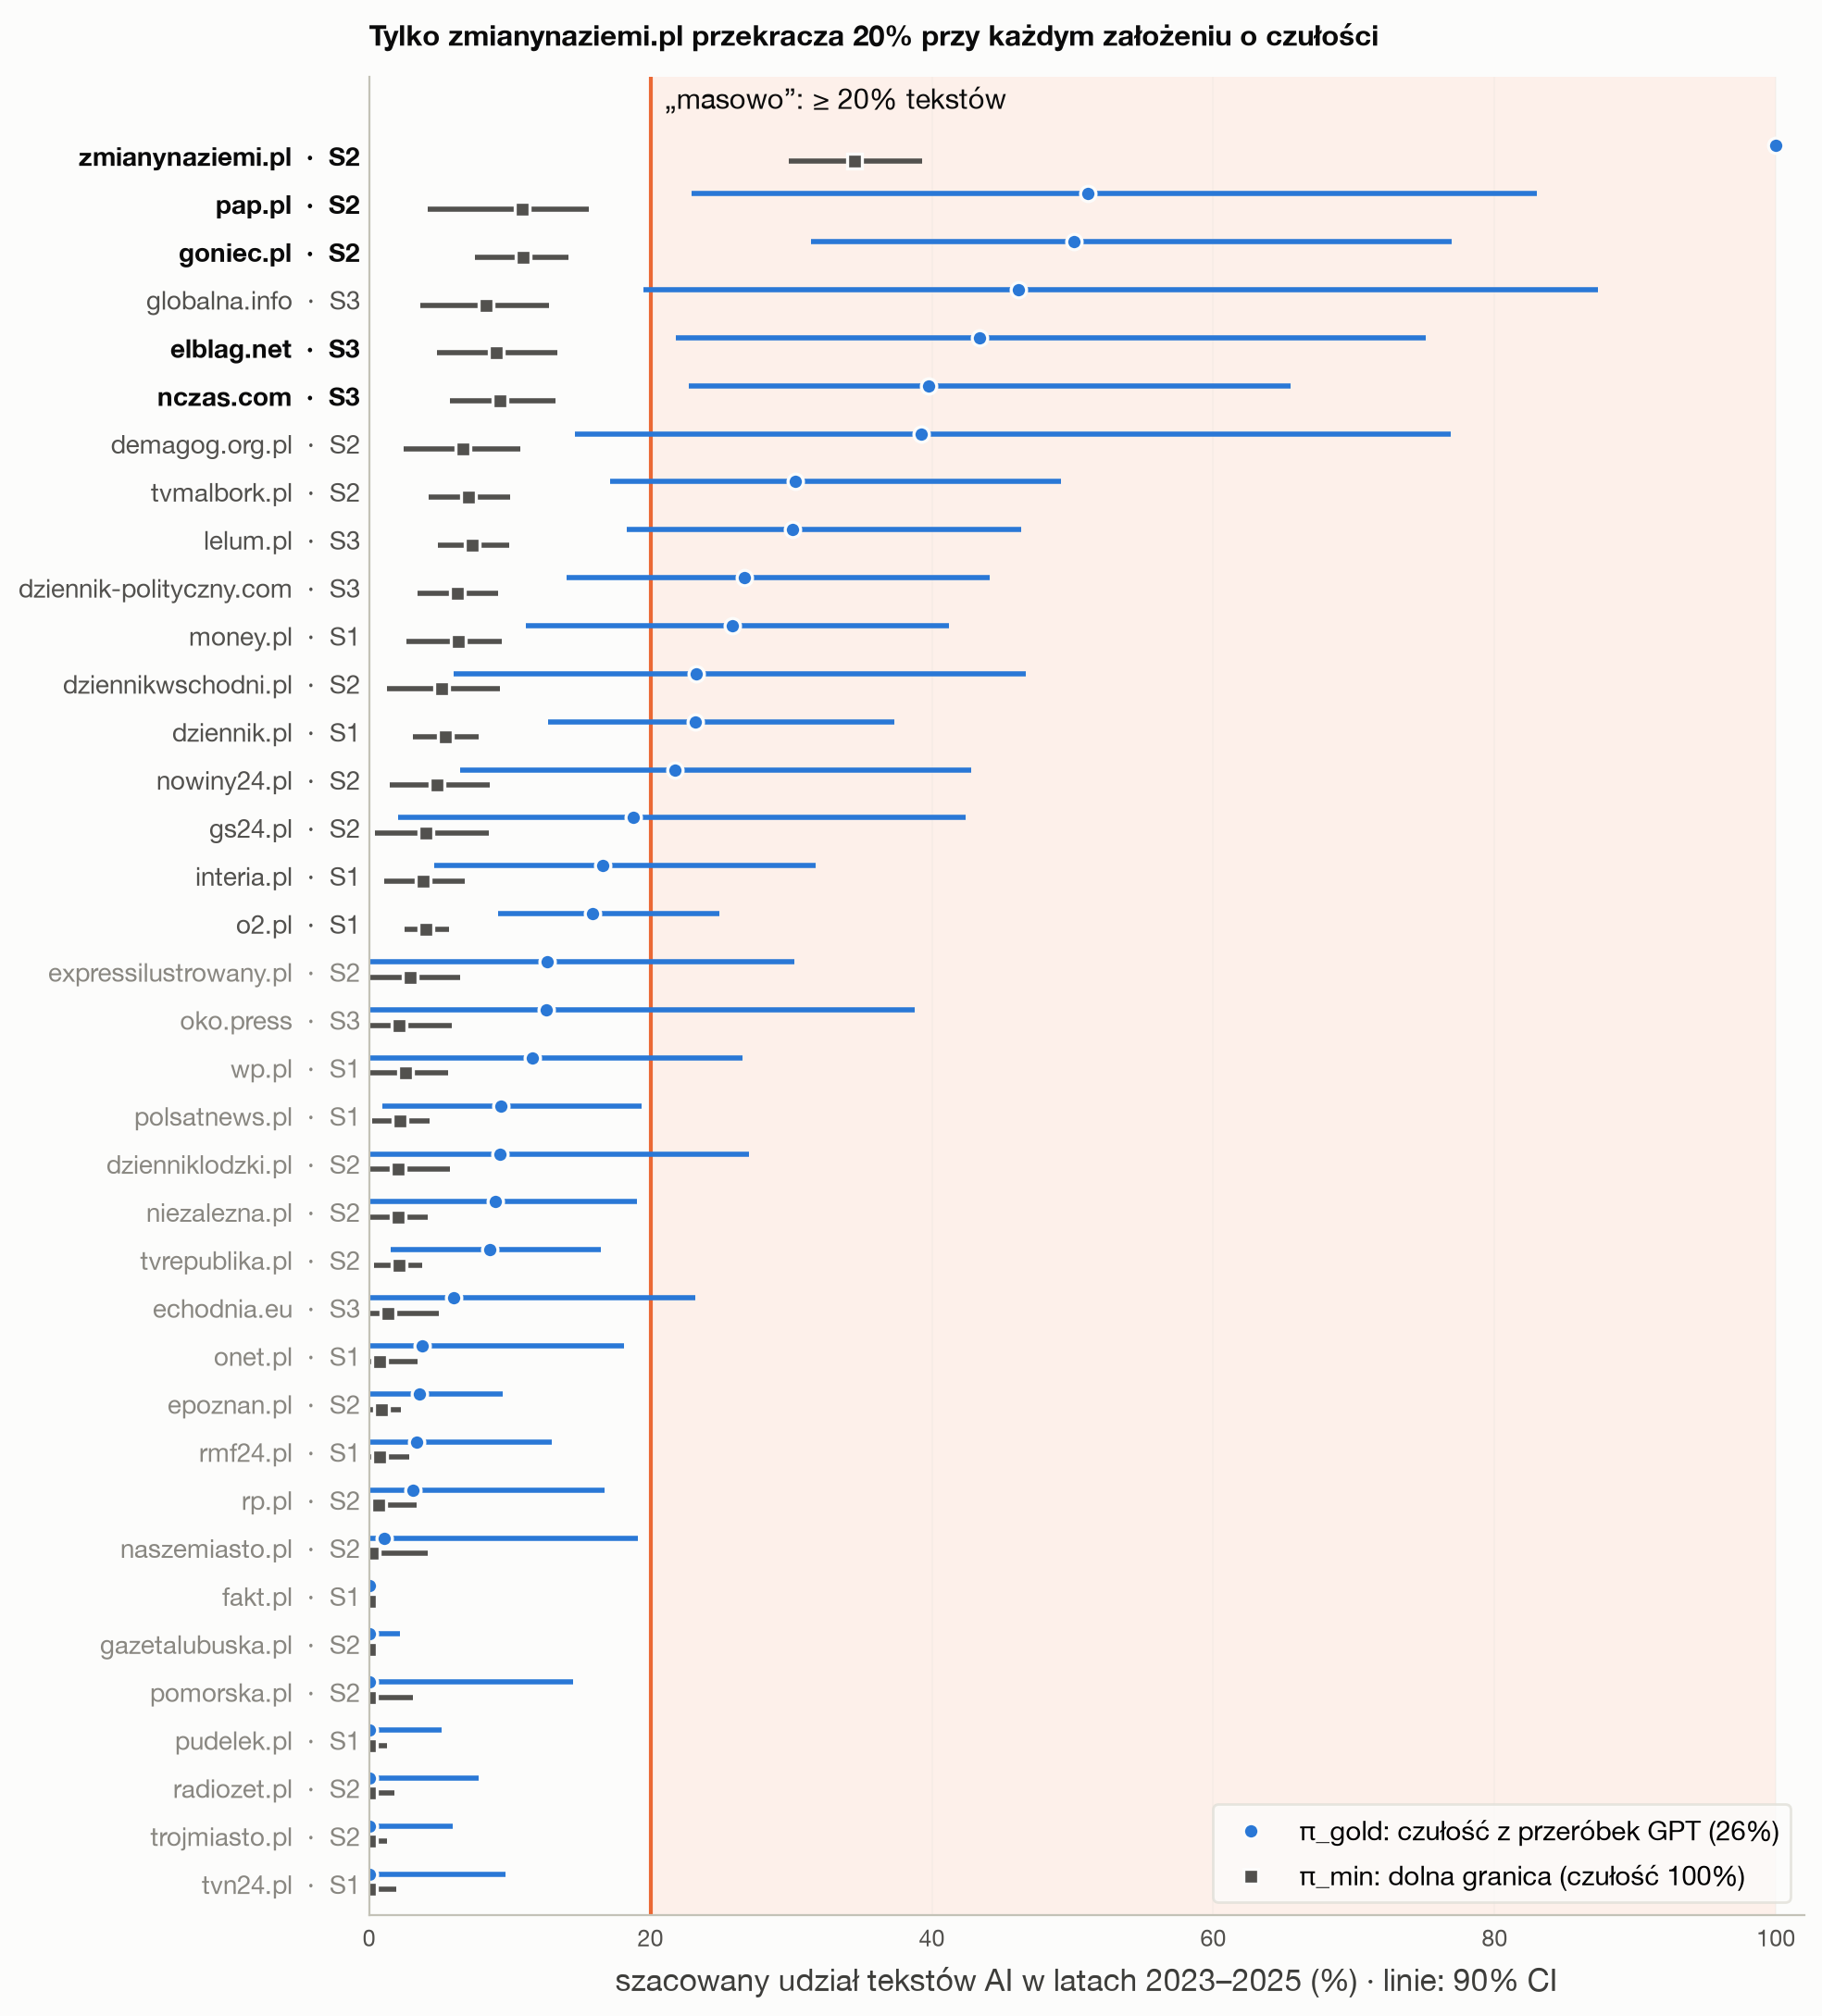
\includegraphics[width=\linewidth,height=0.86\textheight,keepaspectratio]{fig06_forest.png}
\caption{\pimin{} i \pigold{} z 90\% CI dla 37 porównywanych serwisów (dolny koniec przedziału jest jednostronną granicą 95\%). Pogrubione nazwy: serwisy „masowe”, szare: bez nadwyżki ponad dryf. Wartości liczbowe są w aneksie.}\label{fig:las}
\end{figure}

Tabela~\ref{tab:grupy} pokazuje podział serwisów na grupy, a rysunek~\ref{fig:las} przedziały dla każdego z nich.

\dom{zmianynaziemi.pl} (S2) jest masowy z mocnymi dowodami. Oznaczonych jest tam 36,5\% tekstów z lat 2023--2025 wobec 3,1\% w latach 2020--2022. Wartość \pimin{} wynosi 34,5\% [29,8; 39,3], czyli co najmniej 29,8\% tekstów musi pochodzić z AI nawet przy idealnym detektorze. \pigold{} przekracza 100\%, więc teksty AI w tym serwisie są łatwiejsze do wykrycia niż nasze przeróbki. Prawdopodobnie są generowane od zera.

\dom{goniec.pl} (S2) jest masowy prawdopodobnie: 5,3\% $\rightarrow$ 15,7\%, \pigold{} = 50\% [31; 77], \pimin{} = 11\% [7,5; 14,2]. Wynik jest stabilny we wszystkich wariantach analizy.

Trzy kolejne serwisy też spełniają kryterium w analizie głównej, ale każdy ma słabe miejsce. W \dom{pap.pl} (S2) odsetek oznaczonych wzrósł z 6,0\% do 16,2\% (\pigold{} = 51\% [23; 83]), tylko że poziom bazowy pochodzi z 83 tekstów rozłożonych na trzy lata (51, 17 i 15). W \dom{elblag.net} (S3) mamy 6,6\% $\rightarrow$ 15,0\% (\pigold{} = 43\% [22; 75]), a w \dom{nczas.com} (S3) 3,5\% $\rightarrow$ 12,4\% (\pigold{} = 40\% [23; 66]), przy czym cały sygnał \dom{nczas.com} pochodzi z 41 tekstów z 2024 r. Ile wariantów analizy każdy z tych serwisów przetrwał, pokazuje sekcja~\ref{sec:podsumowanie}.

Dwanaście serwisów ma nadwyżkę ponad dryf, ale nie da się wykazać, że jest masowa. Są wśród nich cztery z S1 (\dom{money.pl}, \dom{dziennik.pl}, \dom{interia.pl}, \dom{o2.pl}) oraz \dom{globalna.info}, które leży tuż pod progiem (dolna granica \pigold{} 19,5\% wobec wymaganych 20\%). Dane wskazują tam na AI w części tekstów, ale nie pozwalają oddzielić kilku procent od kilkudziesięciu. Żaden z największych serwisów (S1) nie jest masowy w analizie głównej. Przy progu zależnym od długości tekstu do grupy „prawdopodobnie” wchodzi co prawda \dom{o2.pl} (sekcja~\ref{sec:dlugosc}), więc ten wniosek zależy od wariantu.

\subsection{Kiedy to się zaczęło}

W czterech serwisach (\dom{zmianynaziemi.pl}, \dom{goniec.pl}, \dom{nczas.com}, \dom{neon24.pl}) wzrost jest skokowy (rys.~\ref{fig:czas}). Przez kilka lat odsetek oznaczonych leży przy FPR (3--7\%), a potem w ciągu jednego roku skacze do 36--76\%. Skoki przypadają na różne lata (\dom{neon24.pl} 2023, \dom{zmianynaziemi.pl} i \dom{nczas.com} 2024, \dom{goniec.pl} 2025), więc nie tłumaczy ich jedno wspólne zdarzenie. Bez ręcznego przejrzenia tekstów nie odróżnimy jednak skoku od zmiany szablonu strony albo działu, z którego crawl pobrał artykuły. W \dom{pap.pl} i \dom{elblag.net} skoku nie ma: odsetek oznaczonych utrzymuje się na umiarkowanie podwyższonym poziomie, 15--16\% w \dom{pap.pl} w latach 2024--2025 i 17\%, potem 11\% w \dom{elblag.net}, przy poziomie bazowym około 6--7\%. Takiego wzorca nie odróżnimy od zmiany szablonu, działu czy profilu tematycznego, więc to najsłabsze przypadki wśród serwisów zaliczonych do masowych.

Reguła uśrednia lata 2023--2025, przez co jest ostrożna wobec serwisów, które przeszły na AI później. Tabela~\ref{tab:rok} pokazuje \pimin{} osobno dla każdego roku.

\begin{figure}[t]
\centering
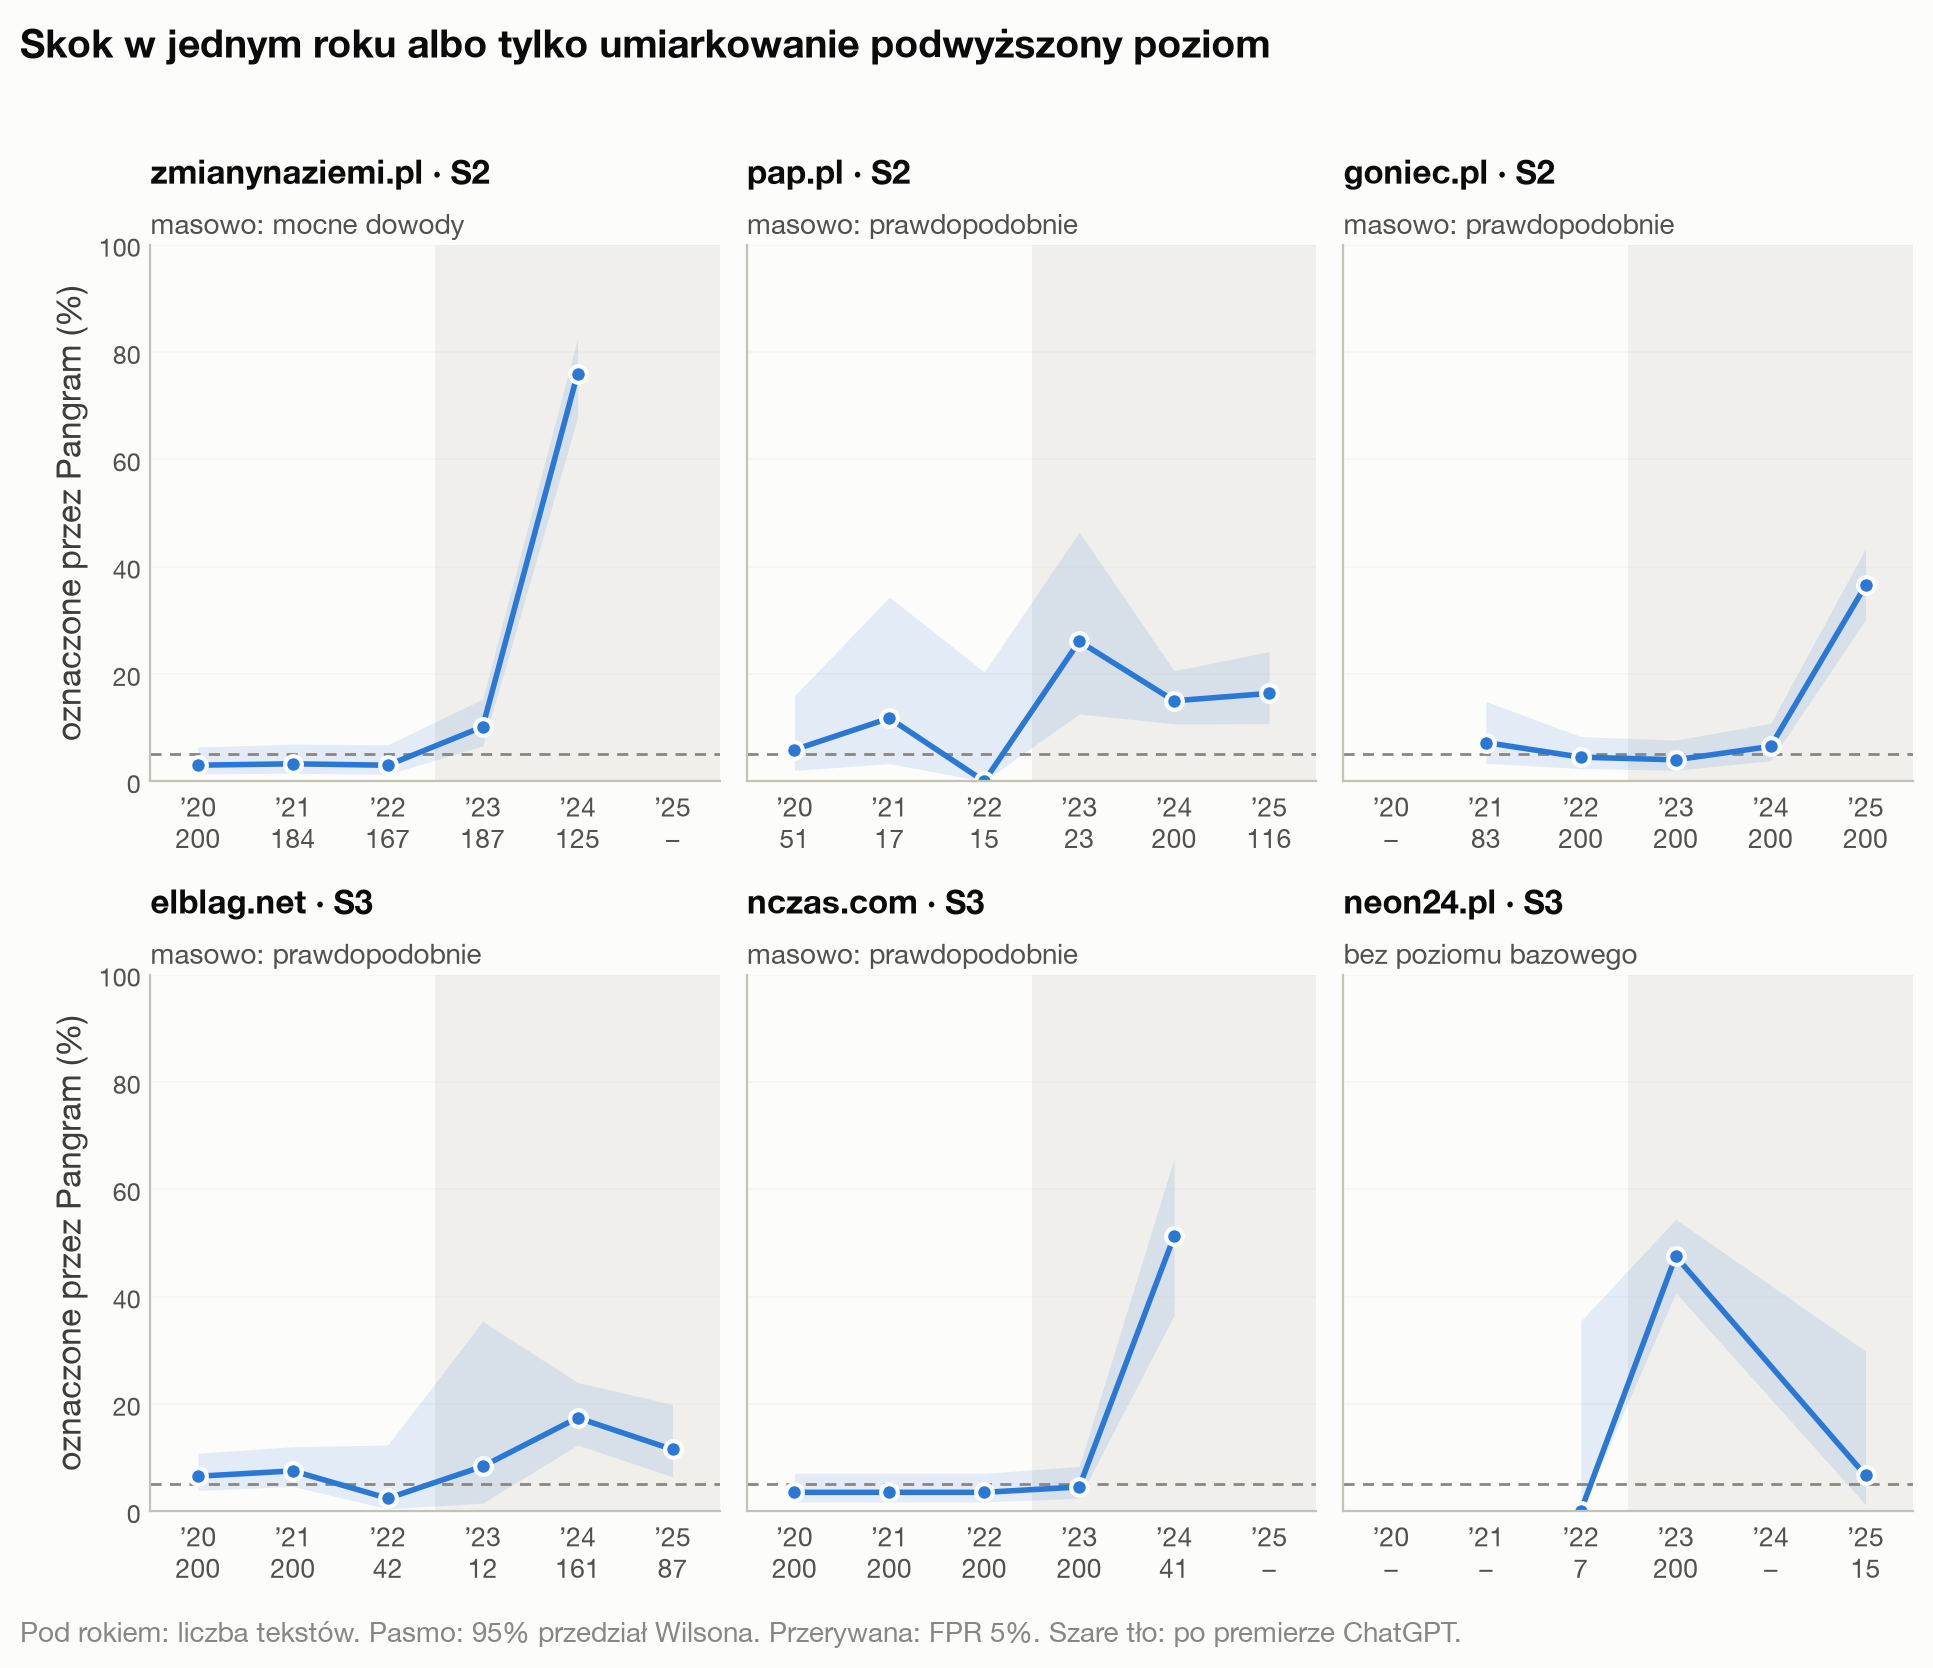
\includegraphics[width=\linewidth]{fig07_timelines.png}
\caption{Odsetek oznaczonych tekstów rok po roku w serwisach „masowych” i w najmocniejszym kandydacie bez porównania przed/po. Pod rokiem liczba tekstów. Pasmo: 95\% przedział Wilsona.}\label{fig:czas}
\end{figure}

\begin{table}[t]
\centering\footnotesize
\caption{Udział AI \pimin{} [90\% CI] w procentach, osobno dla każdego roku. W nawiasie liczba tekstów. Pogrubiony rok skoku.}\label{tab:rok}
\begin{tabular}{@{}lp{3.9cm}p{3.9cm}p{3.9cm}@{}}
\toprule
serwis & 2023 & 2024 & 2025 \\
\midrule
\dom{zmianynaziemi.pl} & 7,3 [3,7; 11,6] (187) & \textbf{75,2 [68,4; 81,1]} (125) & -- \\
\dom{goniec.pl} & 0,0 [0,0; 2,2] (200) & 1,3 [0,0; 5,2] (200) & \textbf{32,9 [27,0; 39,0]} (200) \\
\dom{nczas.com} & 1,0 [0,0; 4,2] (200) & \textbf{49,5 [36,3; 62,6]} (41) & -- \\
\dom{pap.pl} & 21,3 [6,6; 39,4] (23) & 9,6 [2,6; 15,2] (200) & 11,0 [3,2; 18,1] (116) \\
\dom{elblag.net} & 1,9 [0,0; 23,4] (12) & 11,6 [6,3; 17,4] (161) & 5,3 [0,0; 12,3] (87) \\
\bottomrule
\end{tabular}
\end{table}

\subsection{Serwisy bez porównania przed/po}

Te serwisy tylko opisujemy, bez wniosków o udziale AI. Najmocniejszym kandydatem jest \dom{neon24.pl} (S3): 44,7\% [38,2; 51,3] z 215 tekstów z lat 2023--2025 jest oznaczonych. Nawet przy najwyższym poziomie bazowym spośród porównywanych serwisów (11,2\%) dolna granica udziału AI wynosi tam około 38\%. \dom{pikio.pl} i \dom{parezja.pl} mają podobnie wysokie odsetki, ale z 16 i 10 tekstów, więc nie można im ufać. \dom{wpolsce24.tv} ma 4,2\% oznaczonych, czyli poniżej FPR.

\section{Analizy odporności}\label{sec:odpornosc}

Sprawdzamy, czy lista serwisów masowych zmienia się, gdy zmienimy decyzje, które mogły być inne. Rysunek~\ref{fig:odpornosc} zbiera dziewięć wariantów analizy.

\begin{figure}[t]
\centering
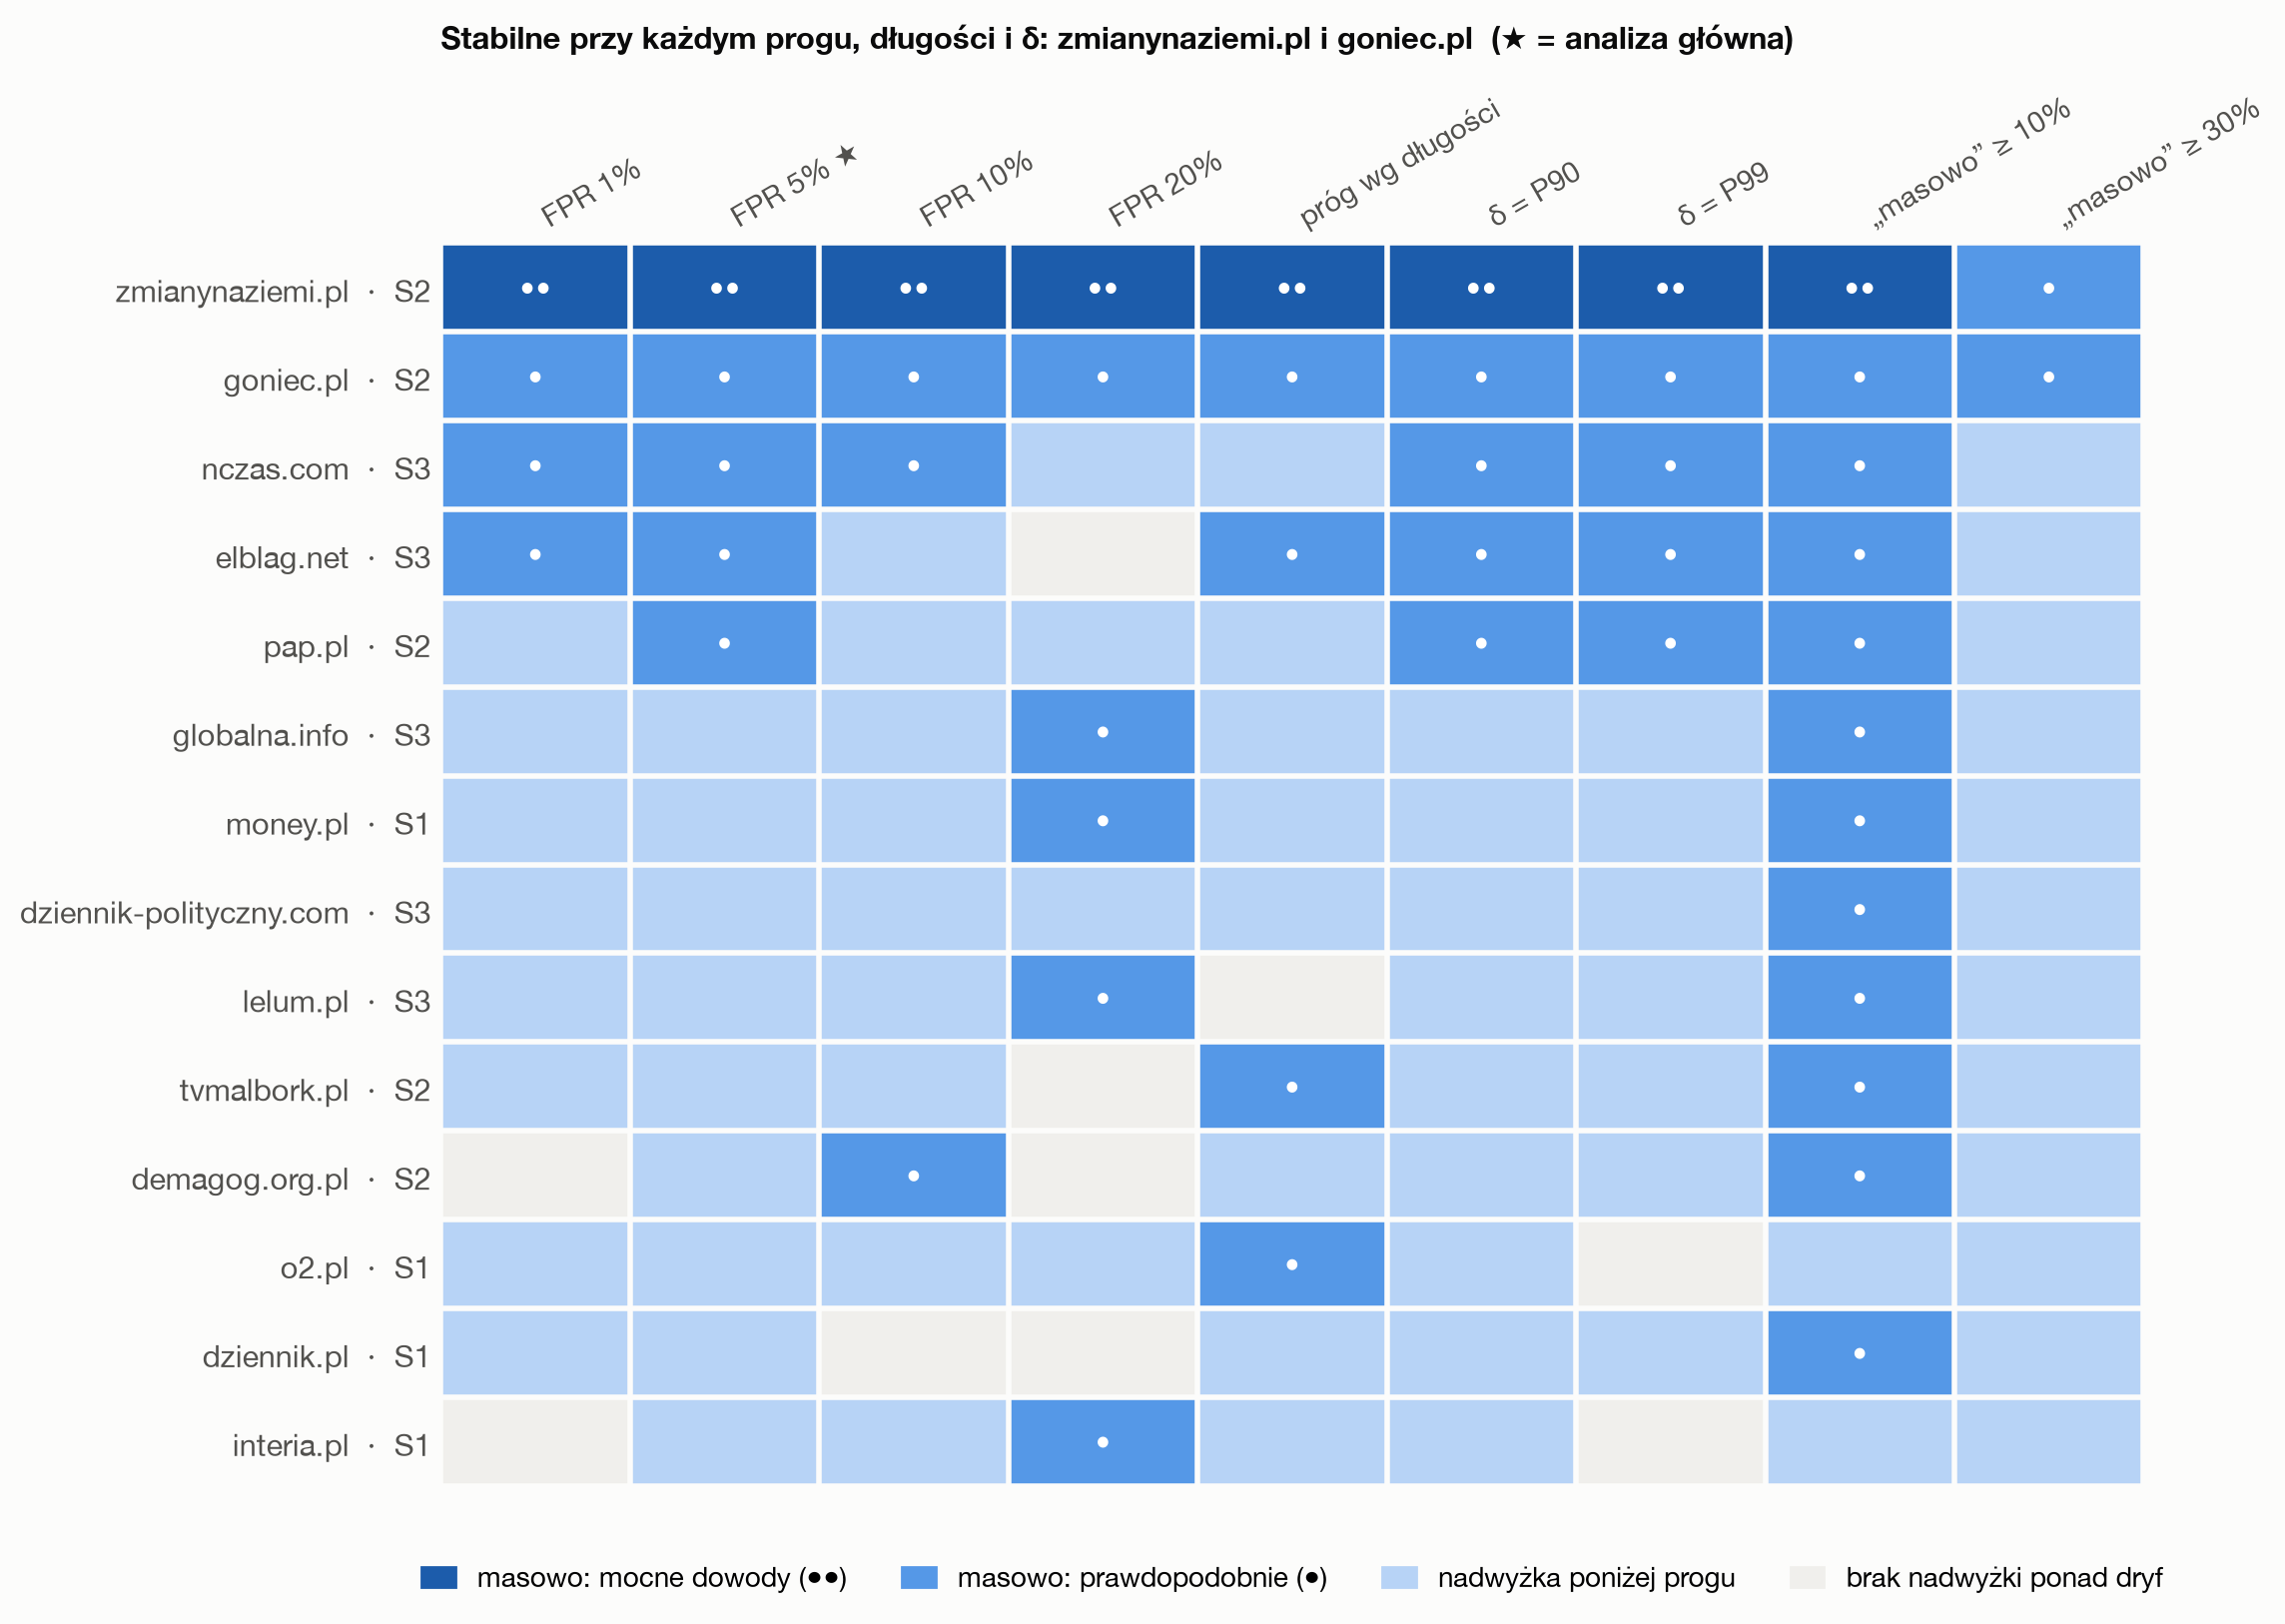
\includegraphics[width=\linewidth]{fig08_robustness.png}
\caption{Grupa każdego serwisu, który choć raz był „masowy”, w dziewięciu wariantach analizy (główna analiza: FPR 5\%).}\label{fig:odpornosc}
\end{figure}

\subsection{Inny próg FPR}\label{sec:fpr}

Dla każdego FPR liczymy od nowa próg, TPR na G2, $\delta$ i szacunki (tab.~\ref{tab:fpr}). \dom{zmianynaziemi.pl} jest masowy z mocnymi dowodami przy każdym progu, a jego \pimin{} rośnie z 28\% do 48\%. \dom{goniec.pl} jest masowy prawdopodobnie przy każdym progu. Przy FPR 20\% jego \pimin{} (26\%) przekracza 20\% jako szacunek punktowy, ale dolna granica już nie, więc nie zalicza się do mocnych dowodów. \dom{nczas.com} jest masowy przy FPR 1, 5 i 10\%, ale nie przy 20\%. \dom{elblag.net} tylko przy 1 i 5\%, a \dom{pap.pl} tylko przy 5\%. \dom{demagog.org.pl} wchodzi wyłącznie przy 10\%, a \dom{globalna.info}, \dom{interia.pl}, \dom{lelum.pl} i \dom{money.pl} wyłącznie przy 20\%. Takich serwisów nie uznajemy za stabilnie masowe, bo ich wynik zależy od progu, który mógł być inny.

Wynik zbiorczy też zależy od FPR. Wraz z nim \pimin{} rośnie (2,0\% $\rightarrow$ 8,2\%), a \pigold{} maleje (21,5\% $\rightarrow$ 11,3\%). Przy FPR 20\% oba szacunki są najbliżej siebie, przy 1\% dzieli je ponad dziesięciokrotna różnica. Przedziały mocno się nakładają, więc nie ma sprzeczności, ale nie ma też jednej stabilnej liczby, i dlatego piszemy o kilku do kilkunastu procentach. Spadek \pigold{} przy niskim FPR pokazuje, że przy surowym progu czułość zmierzona na przeróbkach zaniża czułość na tekstach z serwisów, więc \pigold{} z niskiego FPR jest raczej górną granicą.

\begin{table}[t]
\centering\footnotesize
\caption{Wyniki przy różnych docelowych FPR. Liczby serwisów w grupach: mocne dowody / prawdopodobnie / poniżej progu / brak nadwyżki. Przedziały 95\%.}\label{tab:fpr}
\begin{tabular}{@{}rrrcll@{}}
\toprule
FPR & TPR (G2) & $\delta$ (pp) & grupy & \pimin{} ogółem & \pigold{} ogółem \\
\midrule
1\% & 10\% & 1,5 & 1 / 3 / 10 / 23 & 2,0\% [1,0; 3,5] & 21,5\% [8,4; 53,2] \\
\textbf{5\%} & \textbf{26\%} & \textbf{2,9} & \textbf{1 / 4 / 12 / 20} & \textbf{4,0\% [2,4; 6,1]} & \textbf{18,1\% [9,7; 32,2]} \\
10\% & 45\% & 5,4 & 1 / 3 / 10 / 23 & 5,6\% [3,5; 8,2] & 14,3\% [8,5; 22,9] \\
20\% & 78\% & 9,6 & 1 / 5 / 5 / 26 & 8,2\% [4,8; 12,2] & 11,3\% [6,6; 17,2] \\
\bottomrule
\end{tabular}
\end{table}

\subsection{Długość tekstu}\label{sec:dlugosc}

Wynik Pangrama rośnie z długością tekstu także w latach 2020--2022: żaden tekst ludzki krótszy niż około 360 słów nie przekracza progu. Serwis, który po 2022 r. zacząłby pisać dłużej, miałby więc nadwyżkę bez udziału AI. Mediana długości jednak się nie zmieniła (366 słów przed, 360 po), a wzrost oznaczeń widać w każdym przedziale długości.

Dla sprawdzenia ustawiliśmy próg osobno w ośmiu równolicznych przedziałach długości (każdy na 5\% tekstów z lat 2020--2022 z danego przedziału). TPR na G2 rośnie wtedy do 49\%, a $\delta$ do 3,4 pp. Wynik zbiorczy jest zgodny z głównym: \pimin{} 7,8\% [5,3; 10,4], \pigold{} 16,7\% [11,0; 24,4]. \dom{zmianynaziemi.pl}, \dom{goniec.pl} i \dom{elblag.net} zostają w grupach masowych. \dom{nczas.com} i \dom{pap.pl} spadają do nadwyżki poniżej progu, \dom{lelum.pl} do braku nadwyżki, a \dom{o2.pl} (S1) i \dom{tvmalbork.pl} awansują do „prawdopodobnie”. Poprawka na długość może usuwać część prawdziwego efektu (AI też może wydłużać teksty), więc jest ostrożna.

\subsection{Definicja „masowo” i margines dryfu}

Przy łagodniejszej definicji (co najmniej 10\% tekstów) serwisów masowych jest 12, razem z mocnymi dowodami. Przy ostrzejszej (30\%) są dwa: \dom{goniec.pl} oraz \dom{zmianynaziemi.pl}, który spada wtedy z mocnych dowodów do „prawdopodobnie”, bo dolna granica jego \pimin{} (29,8\%) leży tuż pod 30\%. Liczba serwisów masowych silnie zależy więc od definicji i dlatego podajemy ją zawsze razem z nią.

Margines dryfu z 90., 95. i 99.\ percentyla placebo (2,3; 2,9 i 4,7 pp) nie zmienia listy masowych: to w każdym wariancie te same pięć serwisów, a ich nadwyżki (od około 8 do 33 pp) są dużo większe niż każde $\delta$. Od $\delta$ zależy tylko liczba serwisów z jakimkolwiek sygnałem (14, 12 albo 8 w grupie „poniżej progu”).

\subsection{Czy przedziały dla serwisów mają deklarowane pokrycie}\label{sec:pokrycie}

Reguła masowości opiera się na dolnej granicy przedziału, sprawdzamy więc, czy leży ona poniżej prawdziwego udziału AI w 95\% przypadków. Robimy to na danych sztucznych, dla których prawdę znamy. Wybieramy prawdziwe $\pi$, poziom bazowy, liczby tekstów i czułość, losujemy „zaobserwowane” liczby oznaczonych tekstów, liczymy przedział dokładnie tą samą procedurą co dla serwisów i sprawdzamy, jak często obejmuje prawdziwe $\pi$. Każdy scenariusz (tab.~\ref{tab:pokrycie_sym}) to 1000 powtórzeń. W dwóch ostatnich scenariuszach łamiemy niezależność artykułów (wspólny autor, szablon, temat): wariancja jest trzy razy większa, niż zakłada model.

\begin{table}[t]
\centering\footnotesize\setlength{\tabcolsep}{3pt}
\caption{Pokrycie przedziałów w symulacji. W nawiasach kwadratowych poziom docelowy.}\label{tab:pokrycie_sym}
\begin{tabular}{@{}p{4.2cm}rrrrrr@{}}
\toprule
scenariusz & $\pi$ & $b$ & $n$ przed / po & dolna gr. [95\%] & 5--95 [90\%] & 2,5--97,5 [95\%] \\
\midrule
typowy serwis & 20\% & 5\% & 300 / 300 & 94,9\% & 89,5\% & 95,2\% \\
typowy serwis, więcej AI & 40\% & 5\% & 300 / 300 & 95,4\% & 87,0\% & 93,3\% \\
mało tekstów przed 2023 (jak \dom{pap.pl}) & 20\% & 5\% & 83 / 339 & 94,6\% & 89,8\% & 94,1\% \\
wysoki poziom bazowy (jak \dom{globalna.info}) & 20\% & 10\% & 379 / 336 & 95,2\% & 89,8\% & 95,3\% \\
zgrupowane artykuły (wariancja $\times 3$) & 20\% & 5\% & 300 / 300 & 86,7\% & 69,3\% & 78,4\% \\
zgrupowane artykuły ($\times 3$), więcej AI & 40\% & 5\% & 300 / 300 & 85,0\% & 70,1\% & 78,9\% \\
\bottomrule
\end{tabular}
\end{table}

Gdy artykuły są niezależne, dolna granica z 5.\ percentyla ma deklarowane pokrycie 95\% (94,6--95,4\%), także przy małej liczbie tekstów przed 2023 r. i przy wysokim poziomie bazowym. Cały przedział 5--95 pokrywa prawdę w 87--90\% przypadków. Nieco niższe pokrycie przy dużym $\pi$ dotyczy górnego końca, którego reguła nie używa. Gdy artykuły są od siebie zależne, pokrycie spada: do 85--87\% dla dolnej granicy i do około 70\% dla przedziału 90\%. Dotyczy to każdego przedziału liczonego z odsetków, także zwykłego 95\% (spadek do 78--79\%). Niezależność artykułów jest założeniem, którego nie umiemy sprawdzić, a przed jego złamaniem częściowo chroni nas tylko warunek, że nadwyżka musi przekraczać $\delta$. Dla serwisów z dolną granicą blisko 20\% (\dom{pap.pl}, \dom{elblag.net}, \dom{nczas.com}, \dom{globalna.info}) jest to realne zastrzeżenie. Dlatego w wnioskach większą wagę ma stabilność w wariantach analizy niż pojedyncza dolna granica.

\subsection{Podsumowanie}\label{sec:podsumowanie}

Przy każdym progu FPR, po poprawce na długość, przy każdym $\delta$ i przy definicji 30\% masowe są tylko \dom{zmianynaziemi.pl} (w ośmiu wariantach z mocnymi dowodami, przy definicji 30\% „prawdopodobnie”) i \dom{goniec.pl} (zawsze „prawdopodobnie”). Pozostałe trzy serwisy są masowe tylko w części z dziewięciu wariantów. \dom{nczas.com} w sześciu (wypada przy FPR 20\%, po poprawce na długość i przy definicji 30\%), \dom{elblag.net} też w sześciu (wypada przy FPR 10 i 20\% oraz przy definicji 30\%), a \dom{pap.pl} w czterech (analiza główna, oba alternatywne $\delta$ i łagodniejsza definicja). Nie podajemy ich jako wyniku, tylko jako kandydatów.

\section{Porównanie z detektorami opartymi na Bieliku}

Tę samą procedurę (próg przy FPR 5\% na latach 2020--2022, poziom bazowy serwisu, $\delta$ z placebo) zastosowaliśmy do Binoculars i Fast-DetectGPT na Bieliku 4,5B. Ich czułości na teksty typu GPT nie znamy (dla 1,5B jest bliska FPR), więc liczymy tylko \pimin{} (tab.~\ref{tab:detektory}, rys.~\ref{fig:detektory}).

\begin{table}[t]
\centering\footnotesize
\caption{Ten sam próg (FPR 5\%) dla trzech detektorów. Przedziały dla serwisów 90\%, dla wyniku ogółem 95\%.}\label{tab:detektory}
\begin{tabular}{@{}p{4.6cm}lll@{}}
\toprule
 & Pangram & Binoculars (4,5B) & Fast-DetectGPT (4,5B) \\
\midrule
AUC Śmigiel / gold & 0,80 / 0,88 & 0,85 / 0,56 (1,5B) & 0,80 / 0,49 (1,5B) \\
oznaczone: poziom bazowy $\rightarrow$ 2023--25 & 4,7\% $\rightarrow$ 8,6\% & 5,0\% $\rightarrow$ 6,0\% & 4,9\% $\rightarrow$ 4,5\% \\
\pimin{} ogółem [95\% CI] & 4,0\% [2,4; 6,1] & 1,1\% [0,0; 2,4] & 0,0\% [0,0; 0,5] \\
serwisy z nadwyżką $>\delta$ & 17 & 9 & 2 \\
\dom{zmianynaziemi.pl}: \pimin{} & 34,5\% [29,8; 39,3] & 15,6\% [12,1; 19,4] & 9,7\% [6,7; 13,0] \\
\dom{goniec.pl}: \pimin{} & 10,9\% [7,5; 14,2] & 3,3\% [1,3; 5,1] & 3,8\% [1,9; 5,5] \\
\dom{pap.pl}: \pimin{} & 10,9\% [4,4; 15,5] & 0,0\% [0,0; 1,5] & 0,0\% [0,0; 0,0] \\
\dom{elblag.net}: \pimin{} & 9,0\% [4,8; 13,4] & 8,5\% [5,2; 12,1] & 0,2\% [0,0; 3,0] \\
\dom{nczas.com}: \pimin{} & 9,3\% [5,7; 13,2] & 5,8\% [2,2; 9,7] & 0,0\% [0,0; 1,6] \\
korelacja rang z Pangramem (teksty / nadwyżki serwisów) & 1 / 1 & 0,02 / 0,23 & 0,08 / 0,21 \\
\bottomrule
\end{tabular}
\end{table}

\begin{figure}[t]
\centering
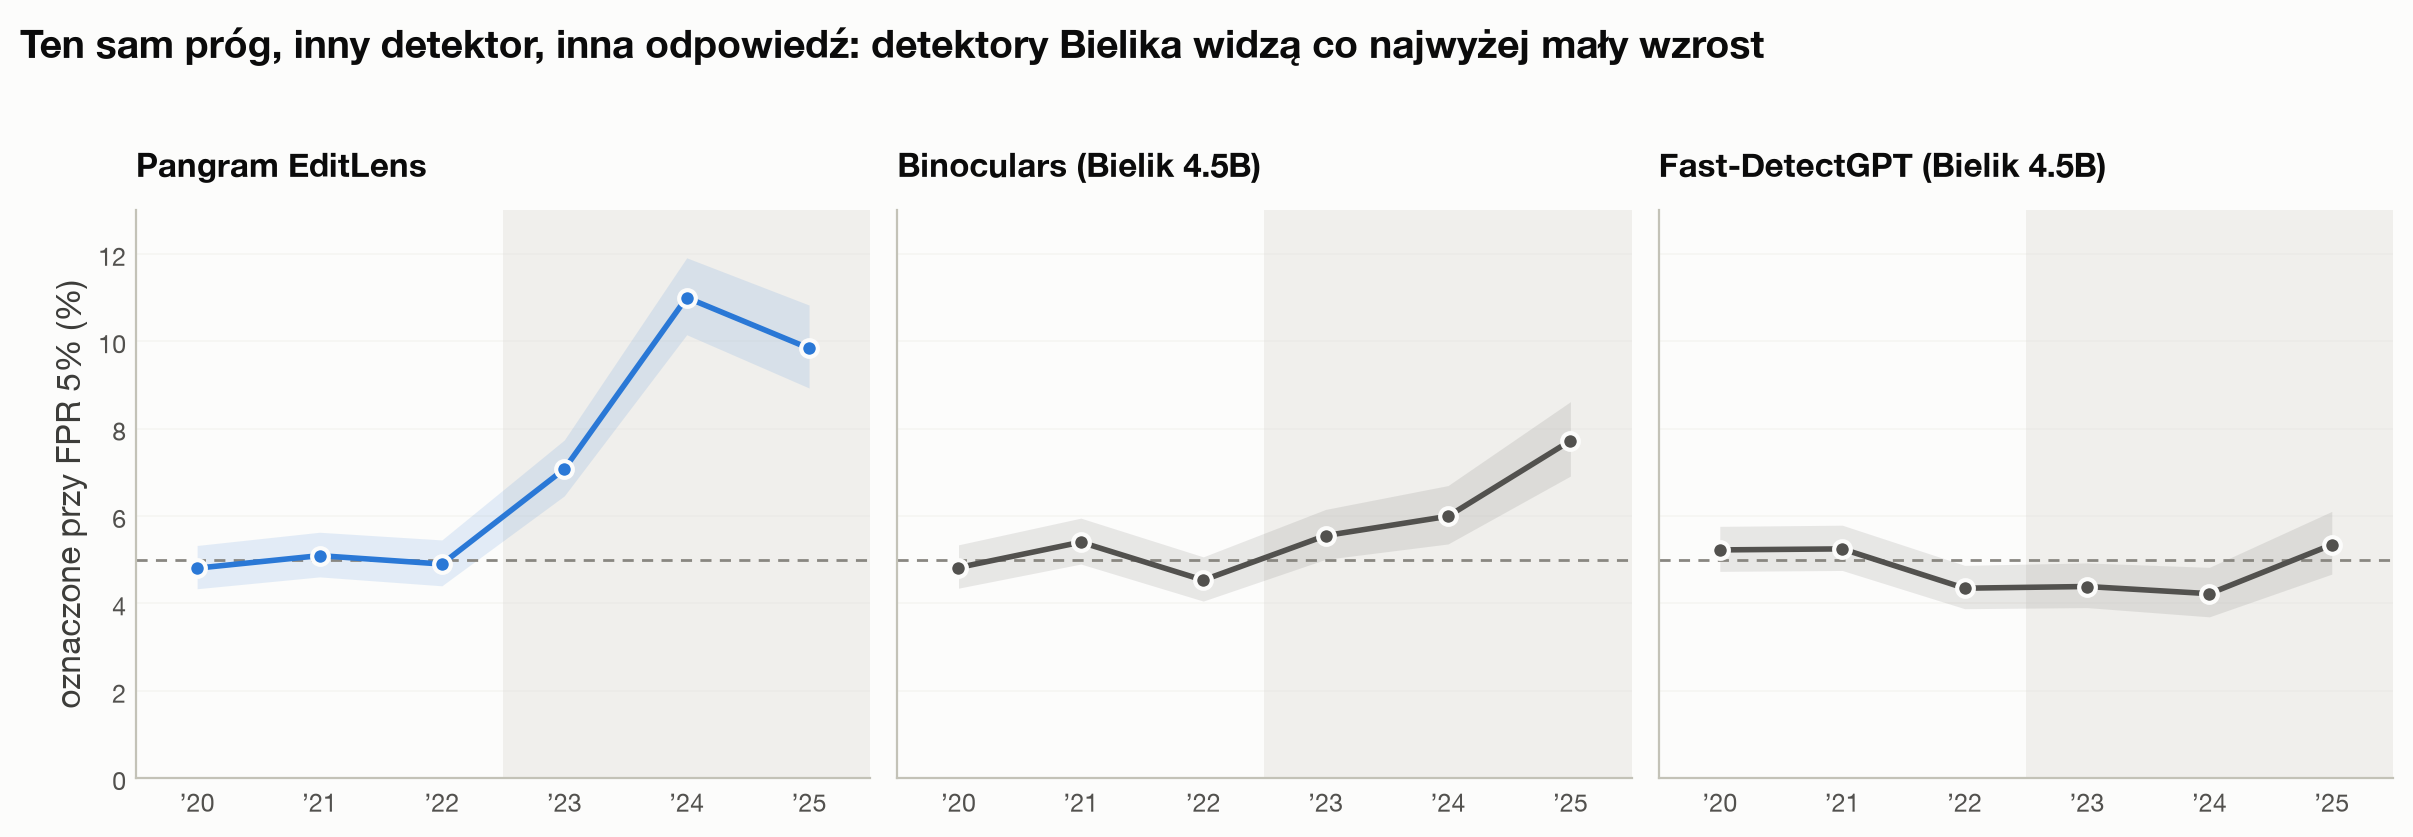
\includegraphics[width=\linewidth]{fig09_detectors_yearly.png}
\caption{Ten sam próg (FPR 5\%) dla trzech detektorów.}\label{fig:detektory}
\end{figure}

Detektory Bielika nie pokazują prawie żadnego wzrostu. Po wynikach walidacji uznajemy, że to skutek ich ślepoty na teksty typu GPT i nie świadczy o braku AI. Mierzą też coś innego niż Pangram: korelacja rang wyników tych samych tekstów wynosi 0,02--0,08. Wyjątkiem jest \dom{zmianynaziemi.pl}, który wyróżnia się we wszystkich trzech detektorach (w Binoculars odsetek oznaczonych rośnie z 1,6\% do 17,0\%). Detektory zbudowane na zupełnie innej zasadzie wskazują więc ten sam serwis, co jest niezależnym potwierdzeniem najmocniejszego wyniku. Skoro Bielik nie widzi przeróbek GPT, a teksty tego serwisu widzi, są one prawdopodobnie innego rodzaju (pisane od zera albo innym modelem), co zgadza się z \pigold{} powyżej 100\% u Pangrama. W \dom{goniec.pl}, \dom{nczas.com} i \dom{pap.pl} detektory Bielika widzą co najwyżej mały wzrost (\pimin{} 0--6\%), ale przy ich ślepocie nie jest to dowód przeciw. Częściowo potwierdza się \dom{elblag.net}: Binoculars daje tam \pimin{} 8,5\%, prawie tyle co Pangram, choć Fast-DetectGPT nie widzi nic.

Wniosek metodologiczny jest taki, że wybór instrumentu zmienia odpowiedź. Gdybyśmy wybierali detektor tylko na podstawie Śmigiela, wzięlibyśmy Binoculars i napisali, że wzrostu prawie nie ma. Walidacja na zbiorze z innej dziedziny wprowadziłaby nas w błąd.

\section{Dyskusja i ograniczenia}\label{sec:ograniczenia}

W naszej próbie 37 polskich serwisów, które da się porównać przed i po 2022 r., jeden (\dom{zmianynaziemi.pl}, S2) publikuje masowo treści, które detektor ocenia jako generowane przez AI, bo co najmniej 29,8\% jego tekstów z lat 2023--2025 pochodzi z AI niezależnie od założeń o czułości. Drugi (\dom{goniec.pl}, S2) prawdopodobnie też: około 50\% przy czułości zmierzonej na przeróbkach, z dolną granicą 31\%, stabilnie przy każdym progu, po poprawce na długość, przy każdym marginesie dryfu i przy definicji 30\%. Trzy kolejne (\dom{elblag.net}, \dom{nczas.com}, \dom{pap.pl}) traktujemy jako kandydatów. Poza porównaniem mocną poszlaką jest \dom{neon24.pl} (S3). Żaden z największych serwisów (S1) nie spełnia kryterium w analizie głównej. W całej próbie udział tekstów AI w latach 2023-2025 szacujemy na od kilku do kilkunastu procent, wyraźnie dopiero od 2024 r.

Ograniczenia, które uważamy za najważniejsze, są następujące.
\begin{enumerate}
\item Czułość znamy dla jednego rodzaju tekstów AI: przeróbek polskich newsów przez jeden model, na 100 parach. Dla tekstów pisanych od zera, innymi modelami, tłumaczonych albo poprawianych przez człowieka może być inna. Podajemy więc przedział od \pimin{} do \pigold{} zamiast jednej liczby. Przedziały dla pojedynczych serwisów są i tak szerokie.
\item Pangram uczono na tekstach angielskich. Na polskich newsach działa (gold, Śmigiel), ale jego wynik zależy od długości tekstu. Uwzględniamy to w analizie odporności, nie w modelu.
\item Zakładamy, że teksty z lat 2020-2022 są ludzkie i że bez AI detektor nie zmienia się w czasie. Placebo pokazuje stabilność w latach 2020-2022, ale nie wyklucza zmiany, która zaczęła się dokładnie po 2022 r. z innego powodu (nowy szablon strony, nowa moda redakcyjna, inne działy w crawlu).
\item Mamy korelację w czasie, nie przyczynowość. Nie dysponujemy ręczną oceną ani deklaracjami redakcji, że konkretne teksty wygenerowała AI. Piszemy więc o nadwyżce tekstów, które detektor ocenia jako podobne do AI, i unikamy sformułowania, że serwis „używa AI”.
\item Próba jest celowa, a S3 wybrano jako podejrzane. Osiem serwisów, w tym sześć z S3, nie ma porównania przed/po. Wniosków nie uogólniamy na wszystkie polskie serwisy.
\item Przy 37 serwisach i jednostronnej granicy 5\% w najgorszym przypadku (wszystkie serwisy tuż poniżej progu) około dwóch dolnych granic przekroczyłoby próg przypadkiem. W praktyce ryzyko dotyczy serwisów bliskich progu: \dom{pap.pl}, \dom{elblag.net} i \dom{nczas.com}.
\item Daty publikacji z trafilatury nie zostały zweryfikowane na próbce. Nie usunęliśmy też prawie identycznych tekstów między serwisami jednej sieci wydawniczej (np. Polska Press) ani nie oznaczyliśmy treści szablonowych (komunikaty, krzyżówki, ostrzeżenia pogodowe).
\item Przyczyna znikania serwisów regionalnych z crawla w latach 2024-2025 nie jest wyjaśniona. Analiza wewnątrz serwisów chroni przed jej wpływem na porównanie, ale zmniejsza moc dla tych lat.
\item Przedziały zakładają niezależność artykułów w serwisie. Gdy mają wspólnego autora albo szablon, pokrycie dolnej granicy spada do około 85-87\% (sekcja~\ref{sec:pokrycie}).
\end{enumerate}



\begin{thebibliography}{99}\small
\bibitem{binoculars} Hans, A., Schwarzschild, A., Cherepanova, V., Kazemi, H., Saha, A., Goldblum, M., Geiping, J., Goldstein, T. (2024). \emph{Spotting LLMs With Binoculars: Zero-Shot Detection of Machine-Generated Text}. Proceedings of the 41st International Conference on Machine Learning (ICML), PMLR 235.
\bibitem{fastdetectgpt} Bao, G., Zhao, Y., Teng, Z., Yang, L., Zhang, Y. (2024). \emph{Fast-DetectGPT: Efficient Zero-Shot Detection of Machine-Generated Text via Conditional Probability Curvature}. ICLR 2024.
\bibitem{editlens} Thai, K., Emi, B., Masrour, E., Iyyer, M. (2026). \emph{EditLens: Quantifying the Extent of AI Editing in Text}. ICLR 2026, arXiv:2510.03154.
\bibitem{rogan} Rogan, W. J., Gladen, B. (1978). Estimating prevalence from the results of a screening test. \emph{American Journal of Epidemiology}, 107(1), 71-76.
\bibitem{smigiel} Przybyła, P. i in. (2025). \emph{PolEval 2025 Task 1 Śmigiel: Spotting Machine-Generated Text from LLMs for Polish}. Proceedings of the PolEval 2025 Workshop, s.~5-15.
\bibitem{bielik} Ociepa, K., Flis, Ł., Kinas, R., Wróbel, K., Gwoździej, A. (2025). \emph{Bielik v3 Small: Technical Report}. arXiv:2505.02550.
\bibitem{tranco} Le Pochat, V., Van Goethem, T., Tajalizadehkhoob, S., Korczyński, M., Joosen, W. (2019). \emph{Tranco: A Research-Oriented Top Sites Ranking Hardened Against Manipulation}. NDSS 2019.
\bibitem{trafilatura} Barbaresi, A. (2021). \emph{Trafilatura: A Web Scraping Library and Command-Line Tool for Text Discovery and Extraction}. Proceedings of ACL-IJCNLP 2021: System Demonstrations.
\bibitem{cc} Common Crawl, \url{https://commoncrawl.org}. Lista crawli: \texttt{config/crawls.yaml} w repozytorium.
\bibitem{raid} Dugan, L., Hwang, A., Trhlik, F., Ludan, J. M., Zhu, A., Xu, H., Ippolito, D., Callison-Burch, C. (2024). \emph{RAID: A Shared Benchmark for Robust Evaluation of Machine-Generated Text Detectors}. ACL 2024, arXiv:2405.07940.
\bibitem{liang2025} Liang, W. i in. (2025). Quantifying large language model usage in scientific papers. \emph{Nature Human Behaviour}.
\bibitem{brown2001} Brown, L. D., Cai, T. T., DasGupta, A. (2001). Interval Estimation for a Binomial Proportion. \emph{Statistical Science}, 16(2), 101--133.
\bibitem{wilson1927} Wilson, E. B. (1927). Probable Inference, the Law of Succession, and Statistical Inference. \emph{Journal of the American Statistical Association}, 22(158), 209--212.
\bibitem{hanley2024} Hanley, H. W. A., Durumeric, Z. (2024). Machine-Made Media: Monitoring the Mobilization of Machine-Generated Articles on Misinformation and Mainstream News Websites. \emph{Proceedings of the International AAAI Conference on Web and Social Media (ICWSM)}, 18, 542--556.
\bibitem{liang2024icml} Liang, W. i in. (2024). Monitoring AI-Modified Content at Scale: A Case Study on the Impact of ChatGPT on AI Conference Peer Reviews. \emph{Proceedings of the 41st International Conference on Machine Learning (ICML)}, PMLR 235.
\bibitem{forman2008} Forman, G. (2008). Quantifying counts and costs via classification. \emph{Data Mining and Knowledge Discovery}, 17(2), 164--206.
\bibitem{gonzalez2017} González, P., Castaño, A., Chawla, N. V., del Coz, J. J. (2017). A Review on Quantification Learning. \emph{ACM Computing Surveys}, 50(5), 74:1--74:40.
\bibitem{detectgpt} Mitchell, E., Lee, Y., Khazatsky, A., Manning, C. D., Finn, C. (2023). DetectGPT: Zero-Shot Machine-Generated Text Detection using Probability Curvature. \emph{Proceedings of the 40th International Conference on Machine Learning (ICML)}, PMLR 202.
\bibitem{russell2025} Russell, J., Karpinska, M., Akinode, D., Thai, K., Emi, B., Spero, M., Iyyer, M. (2025). \emph{AI use in American newspapers is widespread, uneven, and rarely disclosed}. arXiv:2510.18774.
\end{thebibliography}

\appendix
\section{Wszystkie porównywane serwisy}

Tabela~\ref{tab:serwisy} zawiera wszystkie 37 serwisów z porównania przed/po. Plik CSV jest w \texttt{docs/preprint/tables/domains.csv}.

\begin{landscape}
\footnotesize
\setlength{\tabcolsep}{4pt}
\begin{longtable}{@{}l c r r r r r l l l@{}}
\caption{Wszystkie porównywane serwisy, posortowane według $\pi_{\mathrm{gold}}$. Odsetki oznaczonych w procentach (FPR 5\%, Pangram), przedziały dla $\pi$ w procentach i na poziomie 90\% (dolny koniec jest jednostronną granicą 95\%). Grupy według reguły z tab.~\ref{tab:regula}. Dla \texttt{zmianynaziemi.pl} odsetek oznaczonych przekracza TPR z G2, więc $\pi_{\mathrm{gold}}$ jest obcięte (sekcja~\ref{sec:estymator}).}\label{tab:serwisy}\\
\toprule
serwis & warstwa & $n$ 2020--22 & oznaczone 2020--22 & $n$ 2023--25 & oznaczone 2023--25 & nadwyżka (pp) & $\pi_{\mathrm{min}}$ [90\% CI] & $\pi_{\mathrm{gold}}$ [90\% CI] & grupa \\
\midrule
\endfirsthead
\toprule
serwis & warstwa & $n$ 2020--22 & oznaczone 2020--22 & $n$ 2023--25 & oznaczone 2023--25 & nadwyżka (pp) & $\pi_{\mathrm{min}}$ [90\% CI] & $\pi_{\mathrm{gold}}$ [90\% CI] & grupa \\
\midrule
\endhead
\bottomrule
\endlastfoot
\texttt{zmianynaziemi.pl} & S2 & 551 & 3,1 & 312 & 36,5 & 33,5 & 34,5 [29,8; 39,3] & $>$100 (obcięte) & mocne dowody \\
\texttt{pap.pl} & S2 & 83 & 6,0 & 339 & 16,2 & 10,2 & 10,9 [4,2; 15,6] & 51,1 [22,9; 83,0] & prawdopodobnie \\
\texttt{goniec.pl} & S2 & 283 & 5,3 & 600 & 15,7 & 10,4 & 10,9 [7,5; 14,1] & 50,1 [31,4; 77,0] & prawdopodobnie \\
\texttt{globalna.info} & S3 & 379 & 9,8 & 336 & 17,3 & 7,5 & 8,3 [3,6; 12,8] & 46,2 [19,5; 87,4] & poniżej progu \\
\texttt{elblag.net} & S3 & 442 & 6,6 & 260 & 15,0 & 8,4 & 9,0 [4,8; 13,4] & 43,4 [21,8; 75,1] & prawdopodobnie \\
\texttt{nczas.com} & S3 & 600 & 3,5 & 241 & 12,4 & 8,9 & 9,3 [5,7; 13,3] & 39,8 [22,7; 65,5] & prawdopodobnie \\
\texttt{demagog.org.pl} & S2 & 575 & 10,8 & 400 & 16,8 & 6,0 & 6,7 [2,5; 10,7] & 39,2 [14,6; 76,9] & poniżej progu \\
\texttt{tvmalbork.pl} & S2 & 534 & 3,6 & 396 & 10,4 & 6,8 & 7,0 [4,2; 10,0] & 30,3 [17,1; 49,2] & poniżej progu \\
\texttt{lelum.pl} & S3 & 540 & 2,0 & 411 & 9,2 & 7,2 & 7,4 [4,9; 10,0] & 30,1 [18,3; 46,4] & poniżej progu \\
\texttt{dziennik-polityczny.com} & S3 & 341 & 3,2 & 419 & 9,3 & 6,1 & 6,3 [3,5; 9,2] & 26,7 [14,0; 44,1] & poniżej progu \\
\texttt{money.pl} & S1 & 115 & 1,7 & 300 & 8,0 & 6,3 & 6,4 [2,7; 9,4] & 25,8 [11,2; 41,2] & poniżej progu \\
\texttt{dziennikwschodni.pl} & S2 & 423 & 5,0 & 203 & 9,9 & 4,9 & 5,1 [1,3; 9,3] & 23,2 [6,0; 46,7] & poniżej progu \\
\texttt{dziennik.pl} & S1 & 581 & 3,4 & 600 & 8,7 & 5,2 & 5,4 [3,1; 7,8] & 23,2 [12,7; 37,3] & poniżej progu \\
\texttt{nowiny24.pl} & S2 & 564 & 5,0 & 241 & 9,5 & 4,6 & 4,8 [1,5; 8,5] & 21,8 [6,5; 42,8] & poniżej progu \\
\texttt{gs24.pl} & S2 & 594 & 5,6 & 181 & 9,4 & 3,8 & 4,1 [0,4; 8,5] & 18,8 [2,1; 42,4] & poniżej progu \\
\texttt{interia.pl} & S1 & 440 & 3,6 & 340 & 7,4 & 3,7 & 3,9 [1,1; 6,8] & 16,6 [4,6; 31,8] & poniżej progu \\
\texttt{o2.pl} & S1 & 600 & 0,8 & 600 & 4,8 & 4,0 & 4,0 [2,5; 5,7] & 15,9 [9,2; 24,9] & poniżej progu \\
\texttt{expressilustrowany.pl} & S2 & 586 & 3,8 & 198 & 6,6 & 2,8 & 2,9 [0,0; 6,5] & 12,6 [0,0; 30,2] & brak nadwyżki \\
\texttt{oko.press} & S3 & 600 & 11,2 & 491 & 13,0 & 1,9 & 2,1 [0,0; 5,9] & 12,6 [0,0; 38,8] & brak nadwyżki \\
\texttt{wp.pl} & S1 & 453 & 4,6 & 337 & 7,1 & 2,5 & 2,6 [0,0; 5,6] & 11,6 [0,0; 26,5] & brak nadwyżki \\
\texttt{polsatnews.pl} & S1 & 600 & 3,2 & 547 & 5,3 & 2,1 & 2,2 [0,2; 4,3] & 9,4 [0,9; 19,4] & brak nadwyżki \\
\texttt{dzienniklodzki.pl} & S2 & 600 & 4,5 & 200 & 6,5 & 2,0 & 2,1 [0,0; 5,7] & 9,3 [0,0; 27,0] & brak nadwyżki \\
\texttt{niezalezna.pl} & S2 & 600 & 3,7 & 600 & 5,7 & 2,0 & 2,1 [0,0; 4,2] & 9,0 [0,1; 19,1] & brak nadwyżki \\
\texttt{tvrepublika.pl} & S2 & 400 & 1,8 & 600 & 3,8 & 2,1 & 2,1 [0,4; 3,8] & 8,6 [1,5; 16,5] & brak nadwyżki \\
\texttt{echodnia.eu} & S3 & 595 & 4,4 & 194 & 5,7 & 1,3 & 1,4 [0,0; 5,0] & 6,0 [0,0; 23,2] & brak nadwyżki \\
\texttt{onet.pl} & S1 & 600 & 7,8 & 599 & 8,5 & 0,7 & 0,7 [0,0; 3,5] & 3,7 [0,0; 18,1] & brak nadwyżki \\
\texttt{epoznan.pl} & S2 & 481 & 1,5 & 600 & 2,3 & 0,9 & 0,9 [0,0; 2,3] & 3,6 [0,0; 9,5] & brak nadwyżki \\
\texttt{rmf24.pl} & S1 & 600 & 4,3 & 572 & 5,1 & 0,7 & 0,8 [0,0; 2,9] & 3,4 [0,0; 13,0] & brak nadwyżki \\
\texttt{rp.pl} & S2 & 600 & 6,3 & 461 & 6,9 & 0,6 & 0,6 [0,0; 3,4] & 3,1 [0,0; 16,7] & brak nadwyżki \\
\texttt{naszemiasto.pl} & S2 & 575 & 5,9 & 196 & 6,1 & 0,2 & 0,2 [0,0; 4,1] & 1,0 [0,0; 19,1] & brak nadwyżki \\
\texttt{fakt.pl} & S1 & 557 & 7,4 & 600 & 5,0 & $-$2,4 & 0,0 [0,0; 0,0] & 0,0 [0,0; 0,0] & brak nadwyżki \\
\texttt{gazetalubuska.pl} & S2 & 582 & 5,0 & 192 & 2,6 & $-$2,4 & 0,0 [0,0; 0,5] & 0,0 [0,0; 2,2] & brak nadwyżki \\
\texttt{pomorska.pl} & S2 & 571 & 4,6 & 200 & 4,5 & $-$0,1 & 0,0 [0,0; 3,1] & 0,0 [0,0; 14,5] & brak nadwyżki \\
\texttt{pudelek.pl} & S1 & 600 & 1,8 & 471 & 1,7 & $-$0,1 & 0,0 [0,0; 1,3] & 0,0 [0,0; 5,2] & brak nadwyżki \\
\texttt{radiozet.pl} & S2 & 600 & 4,7 & 200 & 3,5 & $-$1,2 & 0,0 [0,0; 1,8] & 0,0 [0,0; 7,8] & brak nadwyżki \\
\texttt{trojmiasto.pl} & S2 & 338 & 6,8 & 130 & 3,8 & $-$3,0 & 0,0 [0,0; 1,2] & 0,0 [0,0; 5,9] & brak nadwyżki \\
\texttt{tvn24.pl} & S1 & 600 & 6,8 & 600 & 6,3 & $-$0,5 & 0,0 [0,0; 2,0] & 0,0 [0,0; 9,7] & brak nadwyżki \\
\end{longtable}
\end{landscape}


\end{document}
